% Use only LaTeX2e, calling the article.cls class and 12-point type.

\documentclass[12pt]{article}

% Users of the {thebibliography} environment or BibTeX should use the
% scicite.sty package, downloadable from *Science* at
% www.sciencemag.org/about/authors/prep/TeX_help/ .
% This package should properly format in-text
% reference calls and reference-list numbers.

\usepackage{scicite}

% Use times if you have the font installed; otherwise, comment out the
% following line.

\usepackage{times}

% The preamble here sets up a lot of new/revised commands and
% environments.  It's annoying, but please do *not* try to strip these
% out into a separate .sty file (which could lead to the loss of some
% information when we convert the file to other formats).  Instead, keep
% them in the preamble of your main LaTeX source file.


\usepackage[utf8]{inputenc}
\usepackage{mathtools}

\usepackage{setspace}
\onehalfspacing
%\linespread{-25.9}
%\renewcommand{\baselinestretch}{0.1}

\setlength{\parskip}{0.5\baselineskip}%
\setlength{\parindent}{0pt}%

% The following parameters seem to provide a reasonable page setup.

\topmargin 0.0cm
\oddsidemargin 0.2cm
\textwidth 16cm 
\textheight 21cm
\footskip 1.0cm


%The next command sets up an environment for the abstract to your paper.

\newenvironment{sciabstract}{%
\begin{quote} \bf}
{\end{quote}}


% If your reference list includes text notes as well as references,
% include the following line; otherwise, comment it out.

\renewcommand\refname{References and Notes}

% The following lines set up an environment for the last note in the
% reference list, which commonly includes acknowledgments of funding,
% help, etc.  It's intended for users of BibTeX or the {thebibliography}
% environment.  Users who are hand-coding their references at the end
% using a list environment such as {enumerate} can simply add another
% item at the end, and it will be numbered automatically.

\newcounter{lastnote}
\newenvironment{scilastnote}{%
\setcounter{lastnote}{\value{enumiv}}%
\addtocounter{lastnote}{+1}%
\begin{list}%
{\arabic{lastnote}.}
{\setlength{\leftmargin}{.22in}}
{\setlength{\labelsep}{.5em}}}
{\end{list}}


% Include your paper's title here

\title{Eclipse and Routing Attacks on P2P Networks} 


% Place the author information here.  Please hand-code the contact
% information and notecalls; do *not* use \footnote commands.  Let the
% author contact information appear immediately below the author names
% as shown.  We would also prefer that you don't change the type-size
% settings shown here.

\author
{Péter Garamvölgyi\\
\\
Department of Computer Science and Technology\\
Tsinghua University, Beijing, China\\
\normalsize{garamvoelgyip10@mails.tsinghua.edu.cn}
}

% Include the date command, but leave its argument blank.

\date{}



%%%%%%%%%%%%%%%%% END OF PREAMBLE %%%%%%%%%%%%%%%%



\begin{document} 

% Double-space the manuscript.

%\baselineskip24pt

% Make the title.

\maketitle 



% Place your abstract within the special {sciabstract} environment.

\begin{sciabstract}
The recent years witnessed a push towards a more decentralized computing paradigm. Peer-to-peer networks are a key building block of such systems. Security analysis of distributed applications is often built on the implicit assumptions of perfect information and secure network. This work discusses network-level attacks on Bitcoin's peer-to-peer network. We believe that the insights gained from our analysis are applicable to other systems too, and can help system architects design more secure distributed systems.
\end{sciabstract}


\section{Peer-to-peer systems}

\subsection{Renaissance of the distributed paradigm}

The recent decades have seen the emergence of a new business model that is based on the value derived from data centralization. At the same time, intentional and accidental misuse of personal information have been becoming an increasingly common phenomenon. Notorious examples include NSA's surveillance system and the numerous recent security issues of Facebook. At the same time, centralized systems often suffer from Denial-of-Service attacks, government interference, and a general lack of transparency.

While the ethical significance of these processes is still an open question to society, they have given rise to the renaissance of the distributed paradigm. A peer-to-peer network is the physical realization of this; it is a system where central application servers and data stores are replaced by nodes of equal abilities and rights, often operated by independent parties. Accompanied by open source software, these systems bring new opportunities and challenges. Advantages include higher reliability, fault tolerance and the possibility of distributed governance. The challenges include optimal resource usage, node discovery, and security.

\subsection{Peer-to-peer and decentralized applications}

\textbf{BitTorrent}\cite{BitTorrent} is a peer-to-peer file sharing protocol dating back to 2004. Files are divided into pieces which are in turn shared among peers directly connecting to each other. Different pieces of the same file can be uploaded to and downloaded from multiple hosts simultaneously, in a non-sequential manner. Centralized servers might be used for sharing torrent descriptor files.

\textbf{IPFS} (\emph{"Inter-Planetary File System"})\cite{IPFS} is a peer-to-peer file system built using Distributed Hash Tables (DHT), borrowing many ideas from other systems including BitTorrent and Git. Instead of creating swarms on an on-demand basis (as is the case in BitTorrent), IPFS forms a single global swarm. Files are chunked and distributed among all nodes, with a replication factor based on the actual demand for the file. As a file system, IPFS is content-addressable and immutable: files are accessed by the hash of their content and cannot be changed. Related projects like FileCoin and Storj aim to guarantee file availability by introducing financial incentives for storing chunks.

\textbf{Signal} is an open-source, peer-to-peer communications application and protocol developed by Open Whisper Systems. Signal offers secure end-to-end encrypted messaging, as well as voice and video calls. Centralized servers are used to facilitate contact discovery and initial message routing. Signal is widely regarded as one of the most secure messaging apps today. \cite{SignalSecurity}

\textbf{Tor} (\emph{"The Onion Router"}) \cite{TOR} is a global volunteer overlay network for privacy-preserving communication. The underlying onion routing protocol uses multiple layers of encryption including the destination IP address. The packet is passed through a virtual circuit of multiple, randomly selected relay nodes. While Tor is not inherently peer-to-peer, it can be a building block for privacy-preserving peer-to-peer applications.

\textbf{Solid} (\emph{"Social Linked Data"}) is a recent project started by World Wide Web inventor Tim Berners-Lee. By allowing users to store their own data in so-called pods, with data access by applications granted and revoked explicitly, Solid aims to return data ownership back to the end users.

Finally, \textbf{Bitcoin} \cite{Nakamoto2008} and other decentralized ledger technologies are also prominent examples of distributed peer-to-peer systems. We will discuss these in detail in section \ref{sec:ledgers}.

\subsection{Attacks on peer-to-peer systems}

There have been multiple works systematically evaluating attacks on peer-to-peer networks \cite{P2PSecurityTaxonomy} \cite{P2PAttacks} \cite{P2PAttacks2}. In the following, we adopt the taxonomy discussed in \cite{P2PSecurityTaxonomy}.

\begin{figure}[h!]
\centering
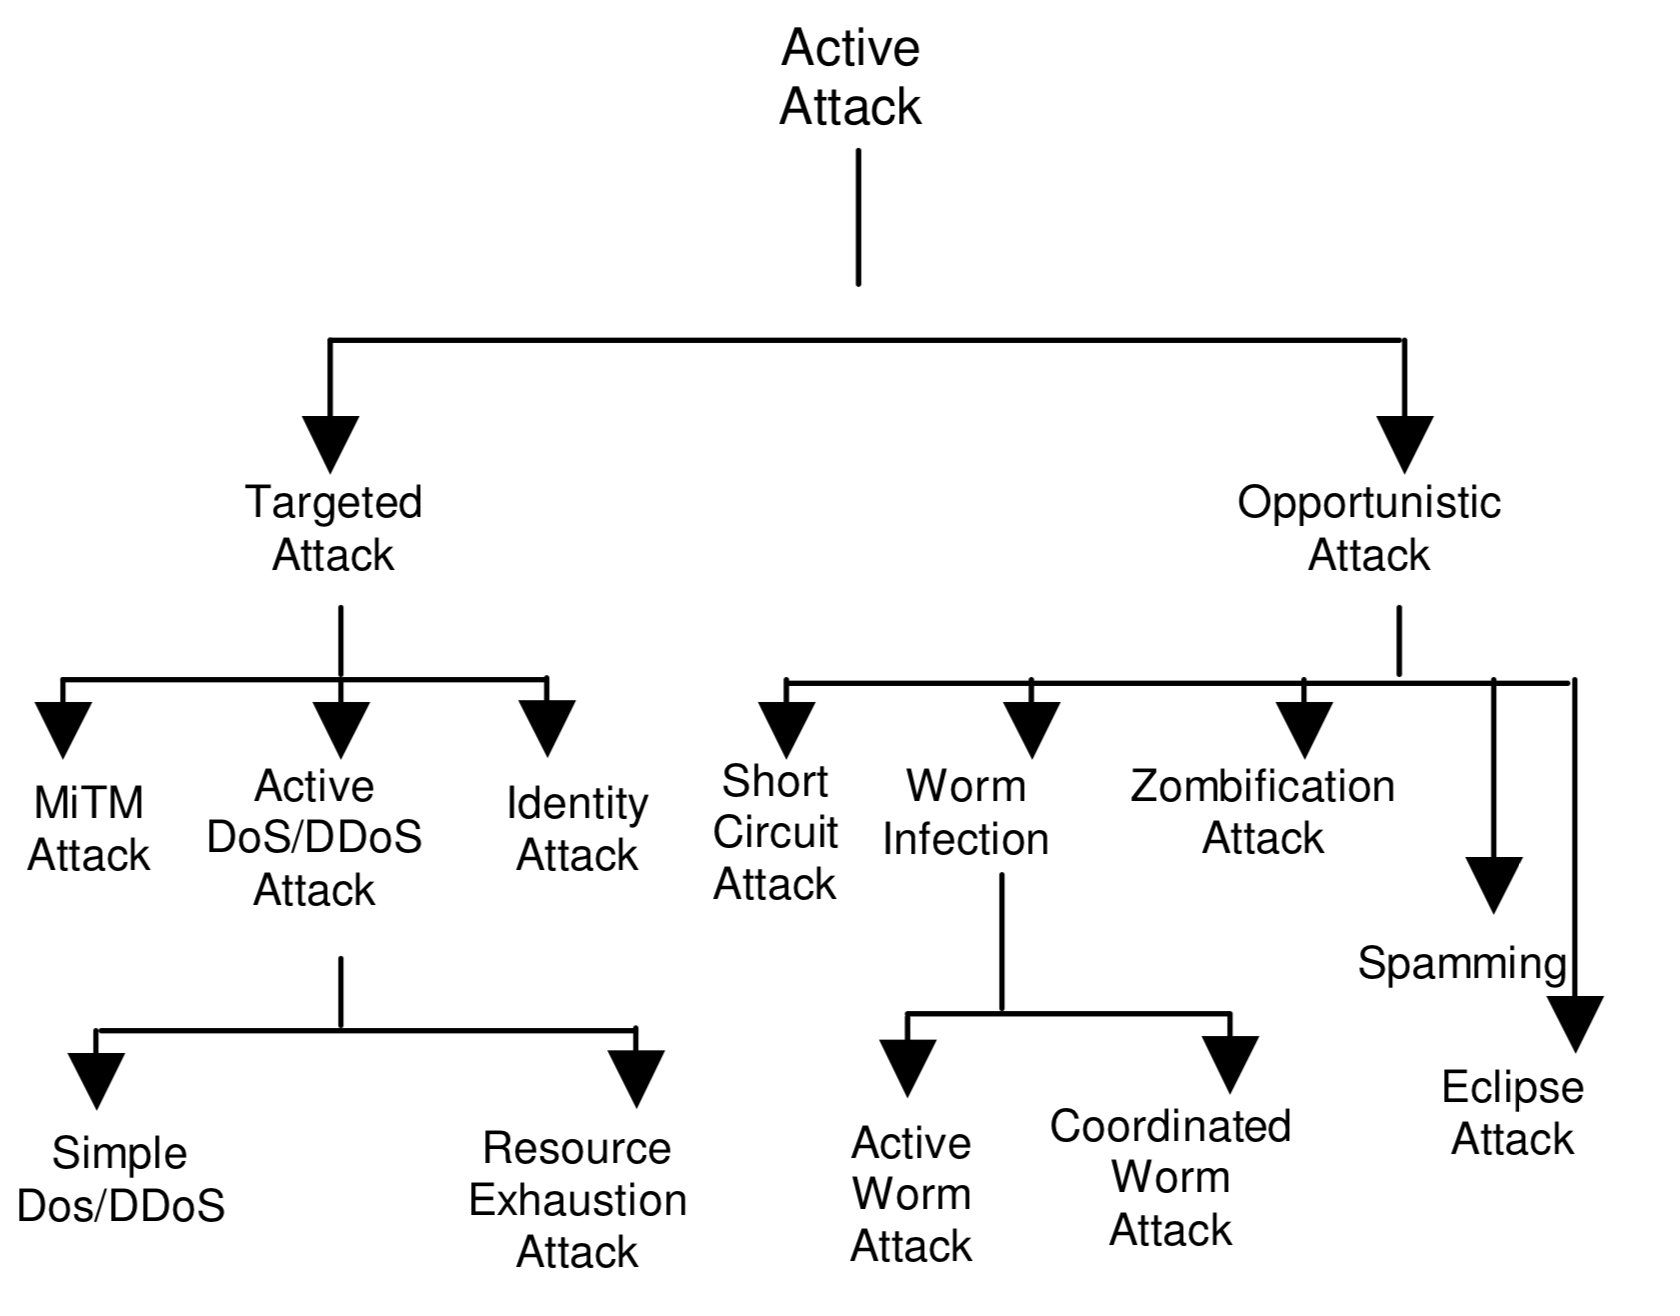
\includegraphics[width=0.6\columnwidth]{images/p2p-active-attack.png}
\caption{Active attacks on peer-to-peer systems \cite{P2PSecurityTaxonomy}}
\label{fig:p2p-active}
\end{figure}

\begin{figure}
\centering
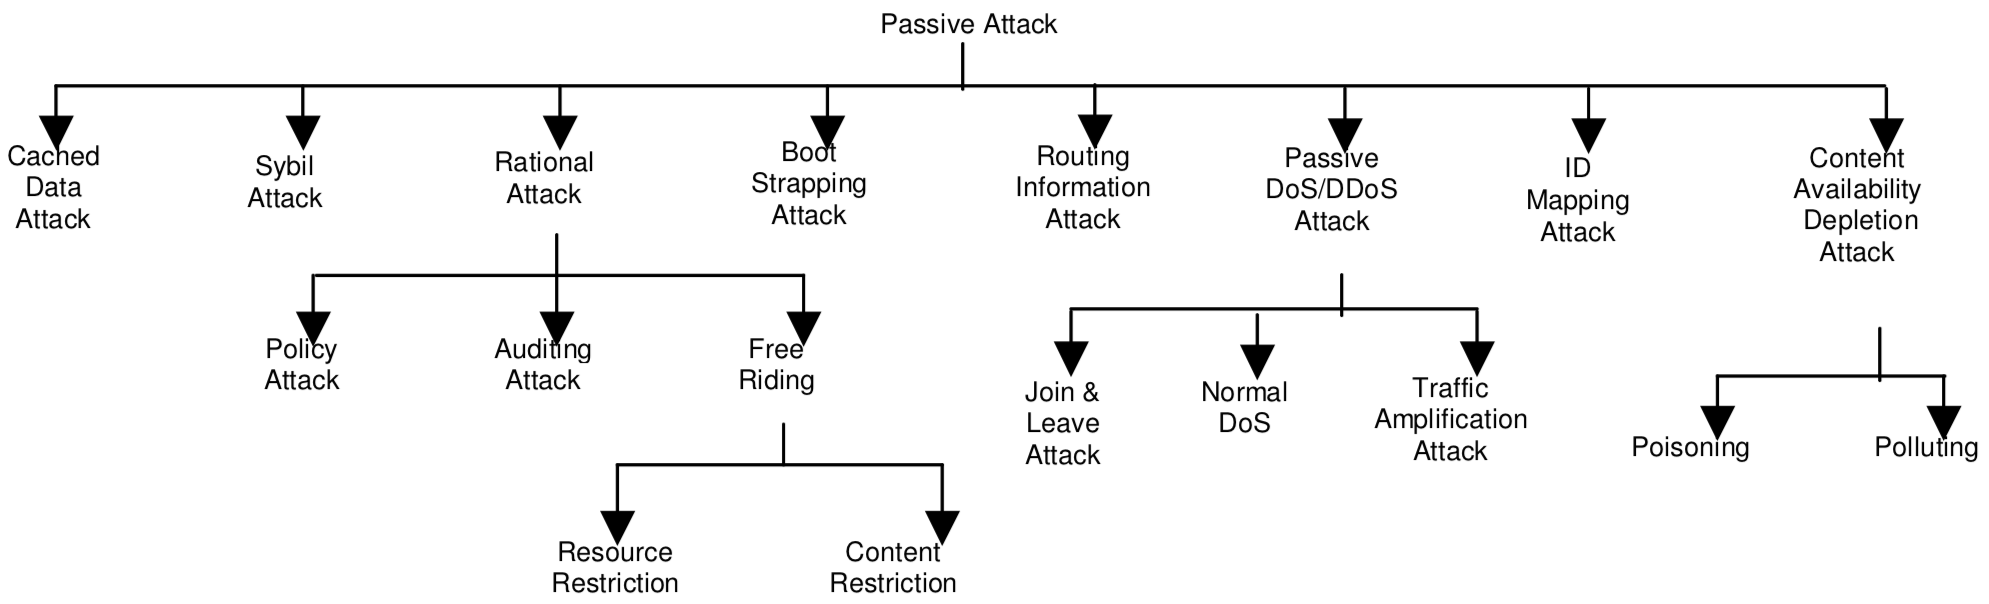
\includegraphics[width=1\columnwidth]{images/p2p-passive.png}
\caption{Passive attacks on peer-to-peer systems \cite{P2PSecurityTaxonomy}}
\label{fig:p2p-passive}
\end{figure}

Attacks can be divided into two main groups:

\begin{enumerate}
    \item \textbf{Active attack}: Main targets are nodes/peers of the network (figure \ref{fig:p2p-active})
    \item \textbf{Passive attack}: Targets the network itself (figure \ref{fig:p2p-passive})
\end{enumerate}

Active attacks include Man-in-the-Middle (MitM), (Distributed) Denial-of-Service (DDoS), identity attacks, zombification attacks, and eclipse attacks, among others.

Passive attacks include sybil attacks, bootstrapping attacks, routing information attacks, traffic amplification attacks, and polluting, among others.

Next, we give a brief description of the attack types relevant to the discussion in this report.

\begin{itemize}
    \item \textbf{Eclipse attack}: "Eclipse attack in P2P network is defined as an attack in which a large number of malicious nodes with some methods compel the legitimate nodes to adopt the malicious nodes as their neighbors so that they can dominate the sets of legitimate nodes."

    \item \textbf{Sybil attack}: "Sybil attack is defined as an attack on uniqueness on identity in which a node dominates the P2P network by obtaining a large number of node identifiers and thus imitating a large number of nodes."

    \item \textbf{Bootstrapping attack}: "When a new node joins the system, it must contact at least one existing node of the system. This process is known as bootstrapping [...] If there is a subnet of malicious nodes around the new node and the new node just bootstraps using one of them then that new node will be effectively a part of the malicious node and be partitioned from the actual network."

    \item \textbf{Routing information attack}: "In the incorrect routing update, a malicious node could corrupt the routing table with incorrect updates to neighbors so that the non-malicious nodes may then start pointing to incorrect nodes or to nonexistent nodes."
\end{itemize}

We encourage the reader to refer to \cite{P2PSecurityTaxonomy} for a more thorough discussion of these attack methods.

The rest of this paper is organized as follows. In section \ref{sec:ledgers}, we give an overview of distributed ledgers, with a focus on network properties and possible attacks. Sections \ref{sec:eclipse}, \ref{sec:partitioning}, and \ref{sec:delay} discuss three prominent network attacks on Bitcoin: eclipse attacks, partitioning attacks, and delay attacks. Finally, section \ref{sec:conclusion} offers some concluding remarks.

\section{Distributed ledgers}
\label{sec:ledgers}

\subsection{The challenge of distributed consensus}

In distributed ledgers, a group of independent, mutually non-trusting nodes would like to maintain a shared state in a secure and robust way. This state can be accounts and corresponding balances, computational states, etc. The state changes are triggered by transactions issued by any node in the network. In its essence, a distributed ledger is a distributed, fault-tolerant state machine.

Fault tolerant state machine replication has been an active area of research since the early 1980s. First, Lamport et al. defined the problem of Byzantine Fault Tolerance \cite{Byzantine}. Later, Fischer et al. proved the theoretical impossibility of distributed consensus under the extreme assumption of asynchrony \cite{FLP}. In 1999, Castro introduced the Practical Byzantine Fault Tolerance (PBFT) algorithm that was the first Byzantine Fault-tolerant approach with practical applicability \cite{PBFT}. PBFT, however, is built on the assumption that the identity and number of participants are known in advance, an assumption that does not hold in dynamic peer-to-peer networks.

Satoshi Nakamoto brought about the next breakthrough by an insightful integration of existing approaches, introducing Bitcoin, the concept of the blockchain, and the new field of Nakamoto consensus \cite{Nakamoto2008}. Blockchains and other distributed ledgers solve state machine replication by maintaining a collection of transactions accepted by the network. In particular, the nodes need to reach consensus on two things:

\begin{enumerate}
    \item \textbf{The validity of transactions}. Whether a transaction is valid must be part of the protocol definition. For instance, in cryptocurrencies, the amount spent by a transaction must not exceed the sender's available balance. Moreover, the same amount cannot be spent twice (so-called double spending). Given a transaction and the current state, the majority of the nodes should either all accept it or all reject it. Given two conflicting transactions A and B, the majority of the nodes should either all accept A or all accept B.

   \item \textbf{The order of transactions}. Most applications (financial transactions, distributed computation) have non-commutative transactions. That is, reordering the same set of transactions will yield different results. Let us look at the following example:

    $$Transaction_A: Alice \xrightarrow{\text{\$200}} Bob$$
    $$Transaction_B: Bob \xrightarrow{\text{\$200}} Claire$$

    Assuming that the initial balance of Bob was \$0, the two possible orderings of these transactions will yield different results: A-B will succeed, while B-A will be rejected, as Bob does not have sufficient balance to send \$200 to Claire.

    Thus, distributed ledgers also need to reach consensus on the full or partial order of all valid transactions. Note that we need not prefer A-B over B-A in the example above; the only requirement is that the majority of nodes agree on either of the two.
\end{enumerate}

Having reached consensus on the validity and (partial) order of transactions, each node can reliably reconstruct the state from any previous state.


\subsection{Bitcoin blockchain}

The first and most famous implementation of Nakamoto consensus is Bitcoin. Bitcoin maintains a cryptographically secure chain of blocks of transactions using longest-chain Proof-of-Work consensus.

\subsubsection{Cryptographically secure chain of blocks}

    Bitcoin organizes transactions into so-called blocks. Each block references the previous one by its hash value, thus creating a tree of blocks. The longest chain rule is used to robustly choose one chain from the root to a leaf as the accepted blockchain.

\begin{figure}[h!]
\centering
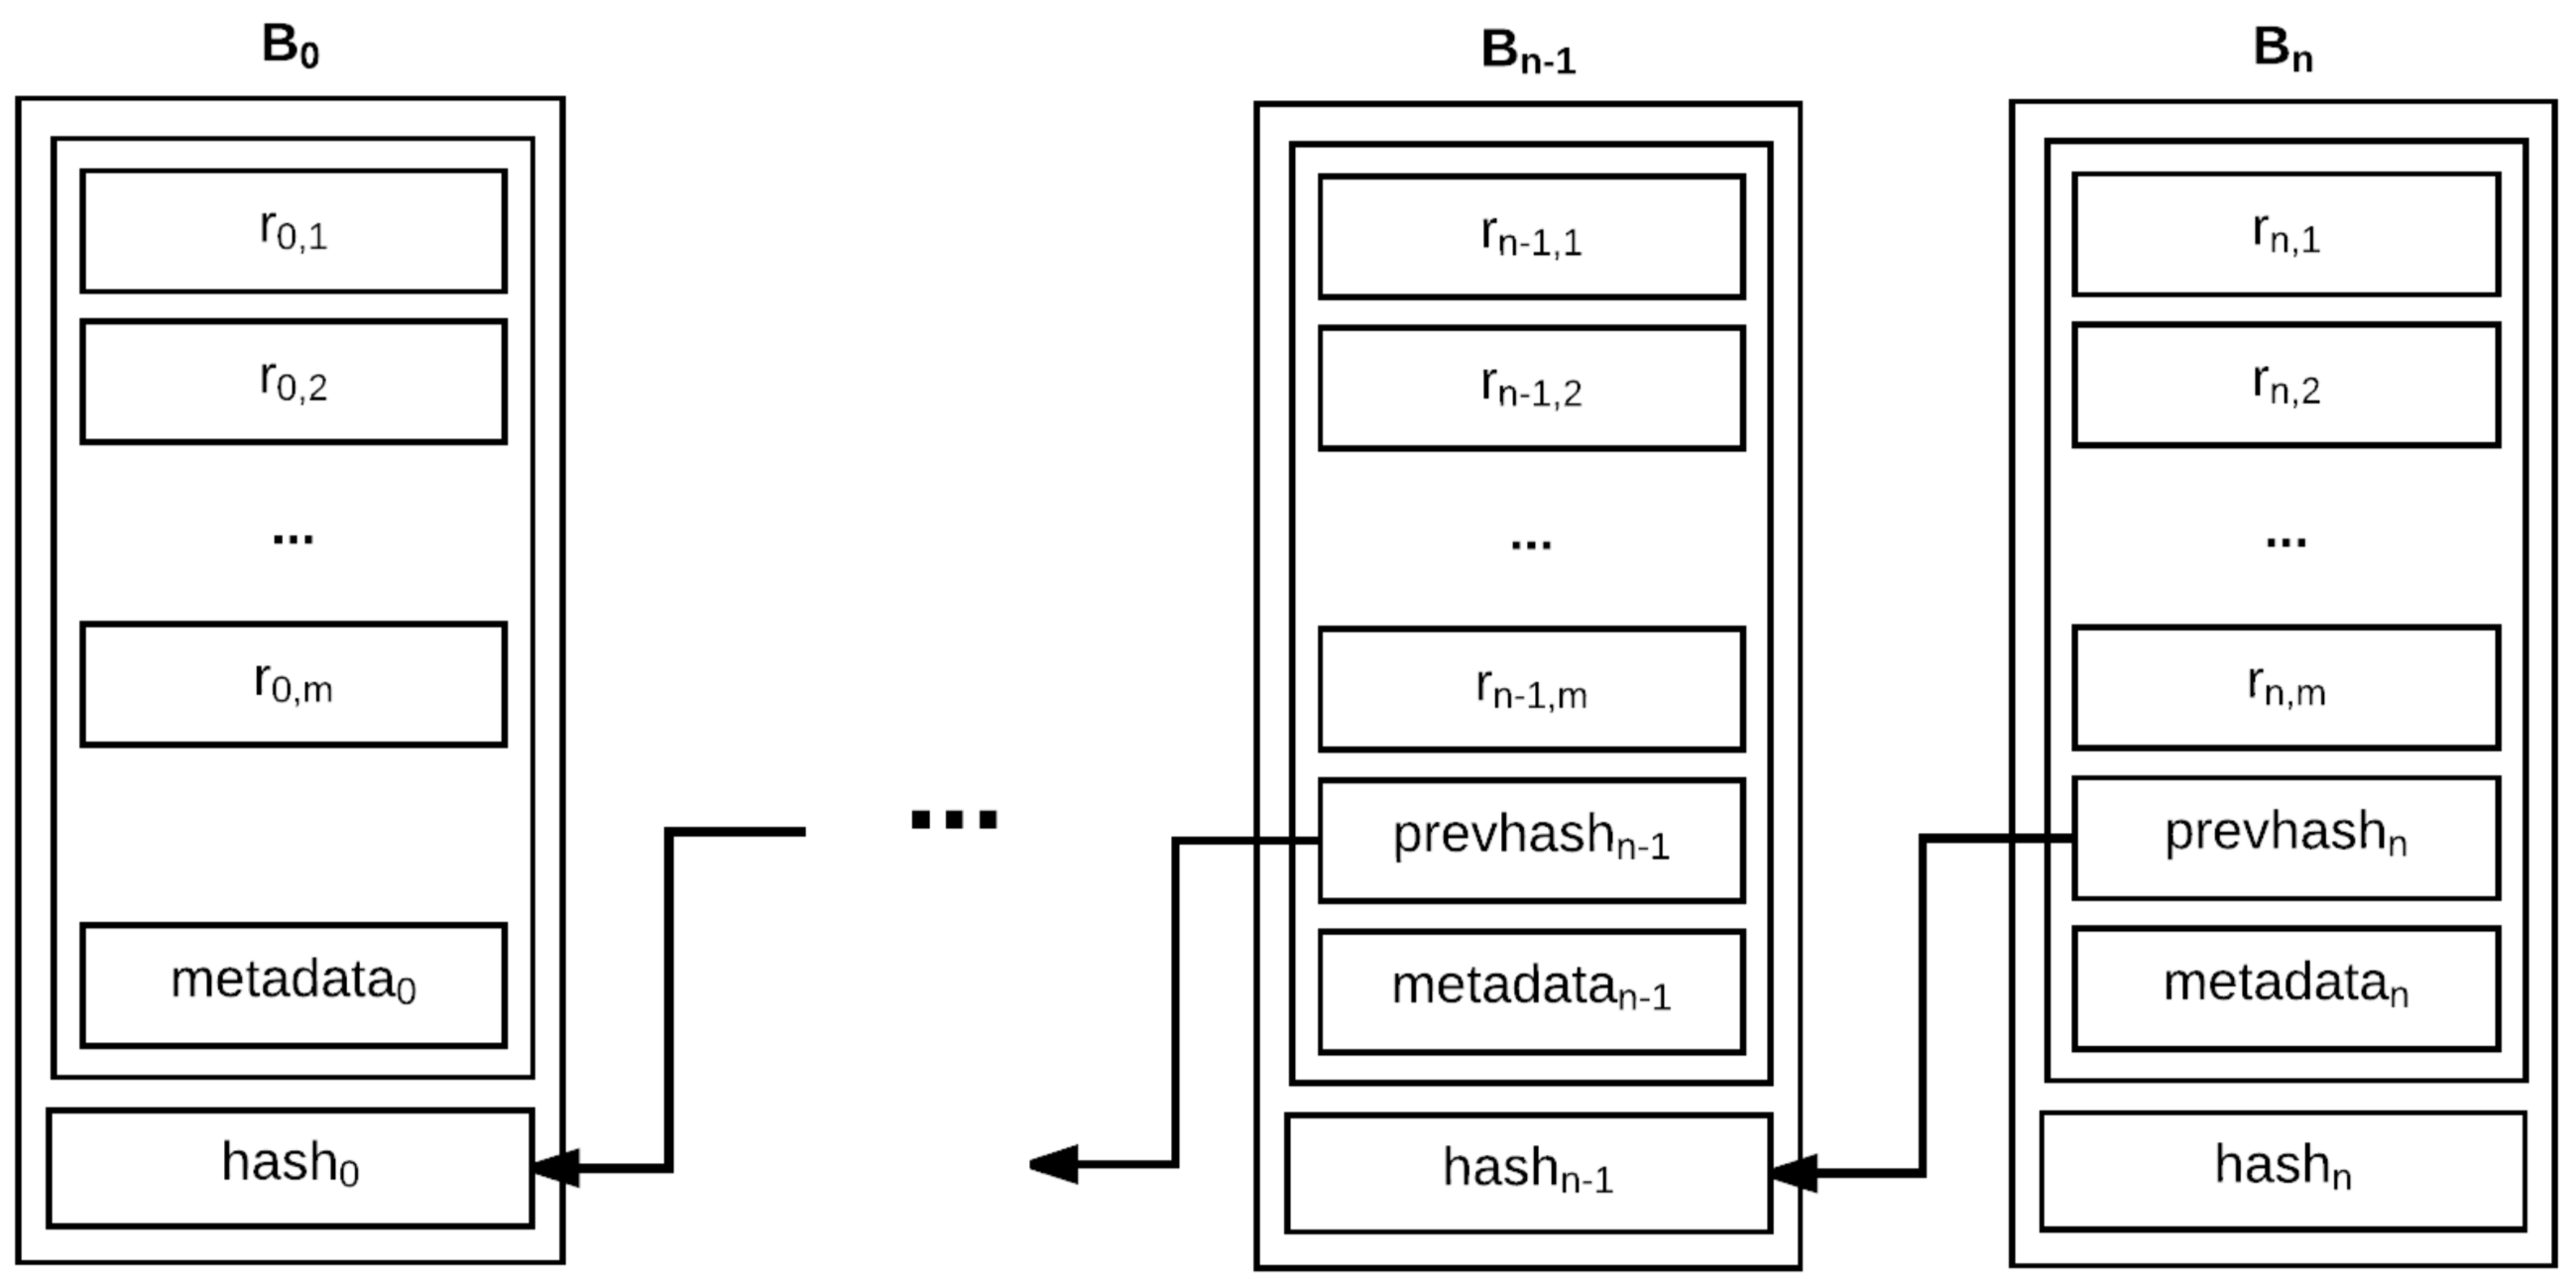
\includegraphics[width=0.7\columnwidth]{images/blockchain.png}
\caption{The blockchain data structure \cite{Garam}}
\label{fig:blockchain}
\end{figure}

    The blockchain data structure (figure \ref{fig:blockchain}) grants both transaction validity and ordering: Blocks accepted by the network are the single-source-of-truth as to which transactions are valid: transactions within the blockchain are valid, while others are either rejected or pending (waiting for approval). At the same time, the blockchain defines a linear order of blocks, while each block also imposes a linear order on transactions within it; together, the blockchain grants full transaction ordering.

\subsubsection{Longest chain rule}

\begin{figure}[h!]
\centering
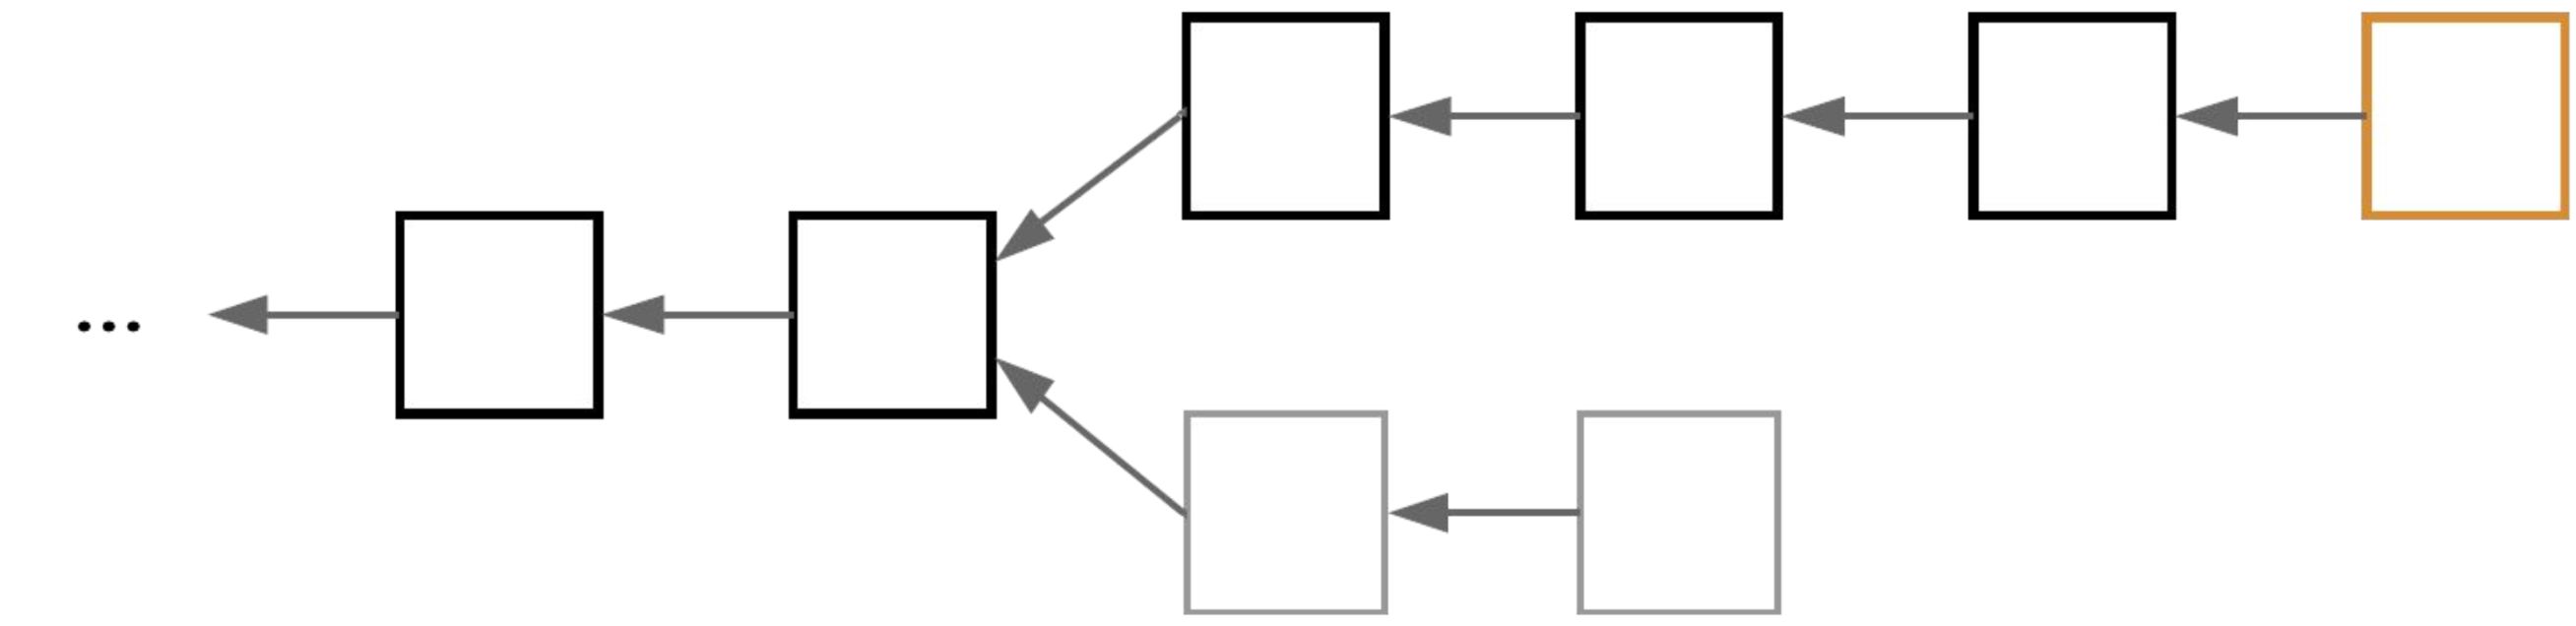
\includegraphics[width=0.7\columnwidth]{images/longest-chain.png}
\caption{Illustration of the longest chain rule in Bitcoin}
\label{fig:longest-chain}
\end{figure}

    Due to network propagation delay or intentional attacks, multiple blocks can reference the same parent block, creating a fork. This is the reason why, strictly speaking, Bitcoin blocks form a tree and not a chain. To reach consensus on the accepted chain, Bitcoin nodes are required to choose the longest from competing chains (figure \ref{fig:longest-chain}). The rationale behind this is that the longest chain is associated with the largest portion of computing power. Other forks (so-called orphan chains) will be discarded.

    The longest chain rule offers probabilistic finality: The probability that a certain block is discarded shrinks exponentially as more and more new blocks are built on top of it.
    
Some work has been done on the security of the longest chain approach and alternative chain selection rules \cite{GHOST}.

\subsubsection{Proof-of-Work (PoW)}

    To create blocks, Bitcoin nodes (miners) are required to solve a computational puzzle called Proof-of-Work. By changing a nonce value in the block header, they need to create a block whose hash has certain characteristics, e.g. a certain number of 0 bits at the front. As Bitcoin uses the cryptographically secure SHA256 hash function, the only way to solve this puzzle is the brute force approach. The block hash and nonce together form the proof that the miner has put a certain amount of computational effort into creating the block.

Proof-of-Work has multiple purposes in Bitcoin:
\begin{itemize}
    \item \textbf{Initial valuation}: As block creation is associated with the creation of new coins, the effort (and electricity) exerted can serve as a reason for why those coins have a non-zero monetary value.
    \item \textbf{Measure of contribution}: The number of blocks created by a miner is proportional to the electricity and hash power invested. Thus, the amount of reward a miner receives is based on the number of blocks it creates.
    \item \textbf{Block delay}: Without PoW, everyone could create blocks all the time. The orphan rate would be huge, and storage would quickly be depleted. Bitcoin sets the block delay at around 10 minutes, ensuring that most of the time all nodes know about all blocks.
    \item \textbf{Leader election}: Leader election mechanisms are often used to decide who issues the next state change (see PBFT, Raft). PoW is effectively a randomized leader election, where each miner issues a portion of blocks proportional to their hash power invested.
    \item \textbf{Sybil resistance}: Distributed voting mechanisms are often used in fault-tolerant systems to decide the validity of the proposed state changes. Bitcoin miners implicitly vote among conflicting blocks by choosing one of them as the parent of the next block. As the computational effort invested into creating a new block has to be tied to a single identity, Bitcoin ensures that each miner's voting power is proportional to their computational power.
\end{itemize}

\subsubsection{Incentives}

    Bitcoin's block reward and transaction fee system encourages rational agents to invest their computational resources into securing the system by creating blocks instead of attacking it. A recent evaluation of Bitcoin's incentive system is presented in \cite{Incentives}.

Bitcoin has many issues ranging from energy inefficiency to unclear governance. However, the combination of the approaches above has been making the system secure for over 10 years now and triggered a thought revolution in distributed consensus.

\subsection{Other distributed ledgers}

\begin{figure}[h!]
\centering
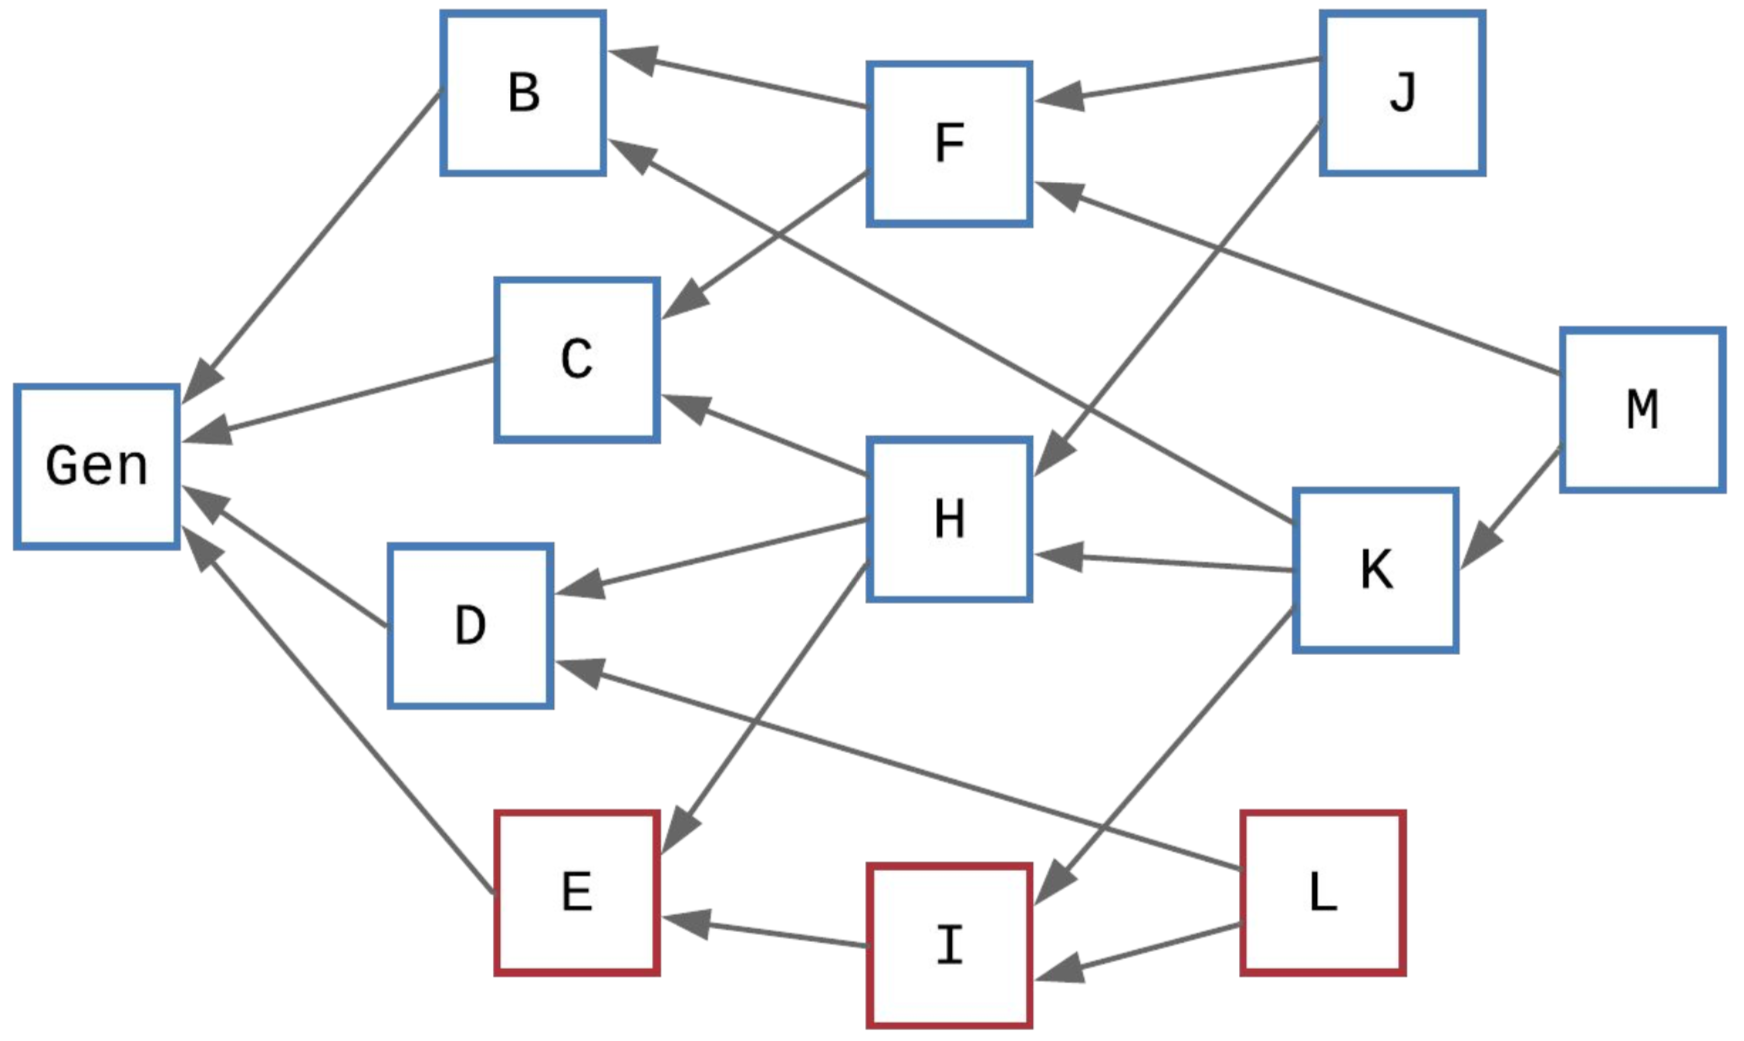
\includegraphics[width=0.6\columnwidth]{images/dag-ledger.png}
\caption{Illustration of a blockDAG \cite{GHOSTDAG}}
\label{fig:dag}
\end{figure}

In the recent years since the publication of Bitcoin in 2008, numerous alternatives have been developed. These new technologies aim to improve on Bitcoin and eliminate its problems by introducing new data structures, consensus mechanisms, and ecosystems. Notable examples include Proof-of-Stake \cite{PoS, PoS2} and DAG-based ledgers \cite{Inclusive, SPECTRE, GHOSTDAG, Conflux, Tangle, Avalanche}.


\subsection{Non-network attacks on distributed ledgers}

Below is a brief description of various attack vectors on distributed ledgers.

\begin{itemize}
    \item \textbf{Double spend}: In a double spend attack, the attacker creates two transactions spending the same funds, one with the merchant as the recipient, the other one moving funds between addresses belonging to the attacker. The attacker first issues the first transaction and waits for the merchant to accept it. Having received the goods or services, the attacker issues the second transaction. If, in the end, the network accepts the second transaction and rejects the first one, the double spend attack was successful. (Also see Finney attack.)

    \item \textbf{Majority attack (51\% percent)}: If an attacker can control the majority of computational power, it can effectively create a longer chain than the honest nodes and control the contents of the blockchain through chain reorganization. An attacker would generally either collude with other existing nodes in the network or involve numerous new nodes thus gaining the majority. There have been several instances of 51\% attacks on smaller blockchains.

    \item \textbf{Sybil attack}: The Bitcoin protocol puts no restriction on the physical nodes and virtual addresses one entity can have. Having multiple physical nodes can be used to perform various network-level attacks like eclipsing. Multiple virtual addresses can be used to gain an unfair advantage in certain applications built on top of blockchains (e.g. voting).

    \item \textbf{DoS and spamming}: An attacker can perform a targeted DoS attack against a group of nodes. An attacker can also attempt to overwhelm the system by issuing a large number of valid transactions. This latter attack is made expensive in systems like Bitcoin by transaction fees. Other systems (IOTA) do not take transaction fees, but require nodes to attach a Proof-of-Work to each transaction instead.

    \item \textbf{Selfish mining}: Selfish mining can let miners gain revenue larger than their proportional effort by strategically withholding certain blocks \cite{SelfishMining}.

    \item \textbf{Forks}: While forks are not an attack vector per se, a hard fork that divides the miners into two groups of roughly equal hash power reduces the security of both chains and makes them susceptible to 51\% attacks.
\end{itemize}

Other attacks include transaction and block malleability attacks, Ice Age, Timejacking, and various smart contract vulnerabilities \cite{BitcoinWeaknesses}.


\subsection{Bitcoin network overview}

Next, we provide a brief overview of Bitcoin's network protocol based on \cite{Heilman2015EclipseAO, RoutingAttacks, BitcoinNetwork}. Further discussion will rely on these details. (Note that due to the evolution of the Bitcoin reference client code base, some of these details might be outdated at the time of reading.)

The Bitcoin peer-to-peer network has the following properties relevant to our discussion:

\begin{itemize}
    \item \textbf{Number of connections}: Nodes have 8 long-lived outgoing connections and up to around 120 unsolicited incoming connections.
    \item \textbf{Security}: The Bitcoin protocol uses neither authentication nor encryption, meaning that confidentiality and integrity are not guaranteed.
    \item \textbf{Peer discovery}: After a restart, nodes try connecting to addresses received previously. Fallback mechanisms include manual specification of peers, DNS seeders whose domain name is hard-coded into the client, and a set of hard-coded IP addresses. Peers can also exchange a list of known addresses by exchanging ADDR messages.
    \item \textbf{Peer information}: Addresses of potential peers are stored in two tables called \emph{tried} and \emph{new}. The former contains addresses to which the node has successfully connected previously. The latter is filled with addresses received from network peers. If the table is full, a probabilistic eviction procedure is executed upon inserting a new address. Both tables are persisted on disk.
    \item \textbf{Peer selection}: New connections are initiated after restarting or when a connection has been dropped. Nodes select one of the two tables based on some probability. Then, the node randomly selects an address from that table with a bias towards fresher addresses. If the node is unable to connect to the selected address, the same process is executed again.
\end{itemize}

The Bitcoin communication protocol defines a set of message types. The following types are relevant to our discussion:

\begin{itemize}
    \item \textbf{ADDR}: Exchange up to 1000 known addresses and the associated timetamps with peers.
    \item \textbf{INV}: Announce a set of new block/transaction hashes to neighbors.
    \item \textbf{GETDATA}: Request block/transaction data to a specific block/transaction hash.
    \item \textbf{BLOCK}: Send block data (in response to GETDATA).
    \item \textbf{TX}: Send transaction data (in response to GETDATA).
\end{itemize}

\section{Eclipse attack}
\label{sec:eclipse}

\subsection{Overview}

Eclipse attacks on Bitcoin were first discussed in detail by Heilman et al. in 2015 \cite{Heilman2015EclipseAO}. Later, similar attacks have been examined on Ethereum \cite{EthereumEclipse}.

\begin{figure}[h!]
\centering
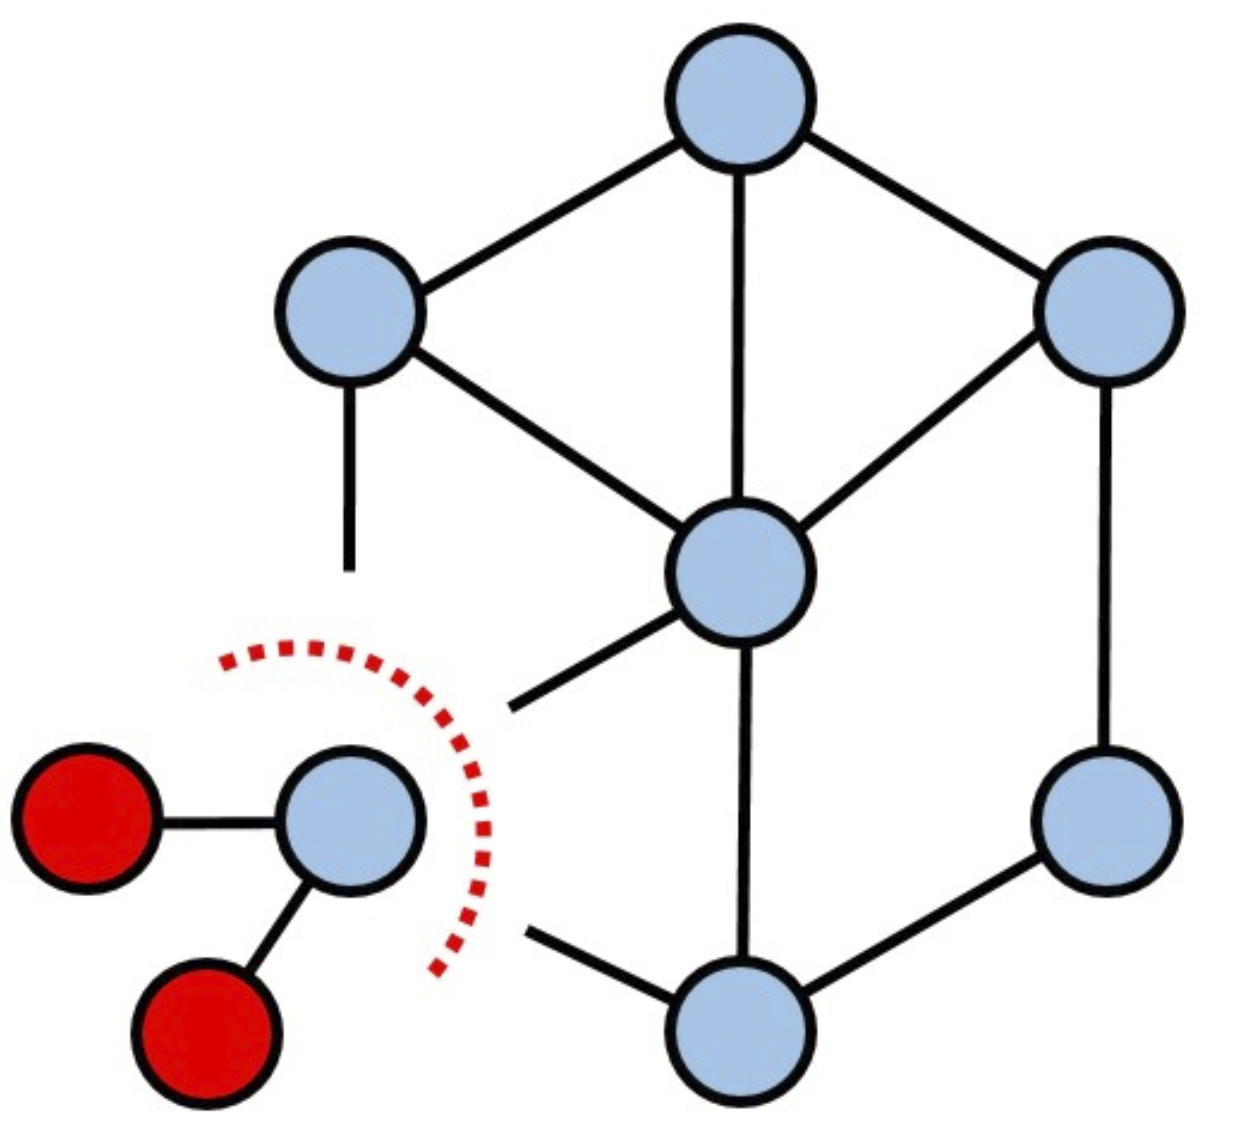
\includegraphics[width=0.4\columnwidth]{images/eclipse.png}
\caption{Illustration of an eclipse attack (image source: https://www.avivz.net)}
\label{fig:eclipse}
\end{figure}

During an eclipse attack on a Bitcoin node, an attacker controlling a sufficient number of IP addresses can occupy all in- and outgoing connections of the victim node with high probability. The eclipsed node's view on the ledger and network can therefore be filtered by the attacker, opening the possibility of other attacks including double spending, Denial-of-Service, and selfish mining.

\subsection{Prerequisites}

To perform an eclipse attack, the attacker must control a sufficient number of IP addresses. The attacker need not control the network infrastructure (in contrast to other network attacks discussed in the subsequent sections).

There are two main types of eclipse attacks based on characteristics of the group of nodes the attacker controls:

\begin{enumerate}
    \item \textbf{Infrastructure attacks}: The attacker is an ISP, large corporation, or government, controlling large contiguous IP prefixes.
    \item \textbf{Botnet attack}: The attacker controls numerous independent nodes in several IP prefixes.
\end{enumerate}

The target node must also have a public IP so that attacker nodes can directly connect to it.

\subsection{Attack process}

To perform an eclipse attack, an attacker executes the following steps.

\begin{enumerate}
    \item \textbf{Populate tried table with attacker addresses}: Addresses associated with unsolicited incoming connections are automatically inserted into the \emph{tried} table. In case the corresponding bucket is full, a probabilistic eviction method is used, which is biased for fresher addresses.
    
Exploiting this mechanism, the attacker can insert its own addresses to the \emph{tried} table by initiating unsolicited incoming connections to the target node.

    \item \textbf{Overwrite addresses in new table}: Addresses from unsolicited ADDR messages will be inserted into the \emph{new} table without connectivity checking. The attacker can use this mechanism to fill the \emph{new} table with addresses of its choice.
    
As addresses controlled by the attacker are considered a scarce commodity, the attacker could use \emph{trash} addresses, e.g. addresses from private IP ranges. This way, the attacker will not waste its resources, but she can still ensure that addresses in the table are useless.

    \item \textbf{Wait for victim node to restart}: Node restarts are relatively common. Outages and software updates often cause node restart, and many of these can be anticipated by the attacker. Alternatively, the attacker can also cause node restart using a DDoS or packet of death attack.

As the authors remark: \emph{Security of the Bitcoin network should not rely on 100\% uptime.}

After restarting, the node will first attempt to form outgoing connections to addresses in the \emph{new} table. However, as these addresses are all \emph{trash}, this will not succeed. Thus, the node will connect to addresses from the \emph{tried} table, choosing addresses with a bias for freshness, thus forming all of its outgoing connections to attacker nodes with high probability.

    \item \textbf{Occupy all incoming connections of victim}: Finally, the attacker can occupy all incoming connections of a node, thus making sure that no other node can connect to the victim.
\end{enumerate}

\subsection{Impact and relevance}

As the authors suggest, eclipse attacks can often be used as building blocks for other attacks. By delaying a node's access to the latest blocks or withholding blocks advertised by it, the attacker can cause revenue loss and engineer block races. At a large scale, these would effectively decrease the network's overall mining power, reducing security. Moreover, eclipsing merchants' nodes would make them susceptible to double spending attacks.

The authors' analysis demonstrates that, with only 4600 botnet addresses, the attacker can fill 98\% of the victim's \emph{tried} table. An infrastructure attack, on the other hand, requires the attacker to control 16000 addresses in 63 groups. Moreover, success probability also relies on the time invested into the attack. In any case, eclipse attacks on Bitcoin nodes remain a practical threat.

\begin{figure}
\centering
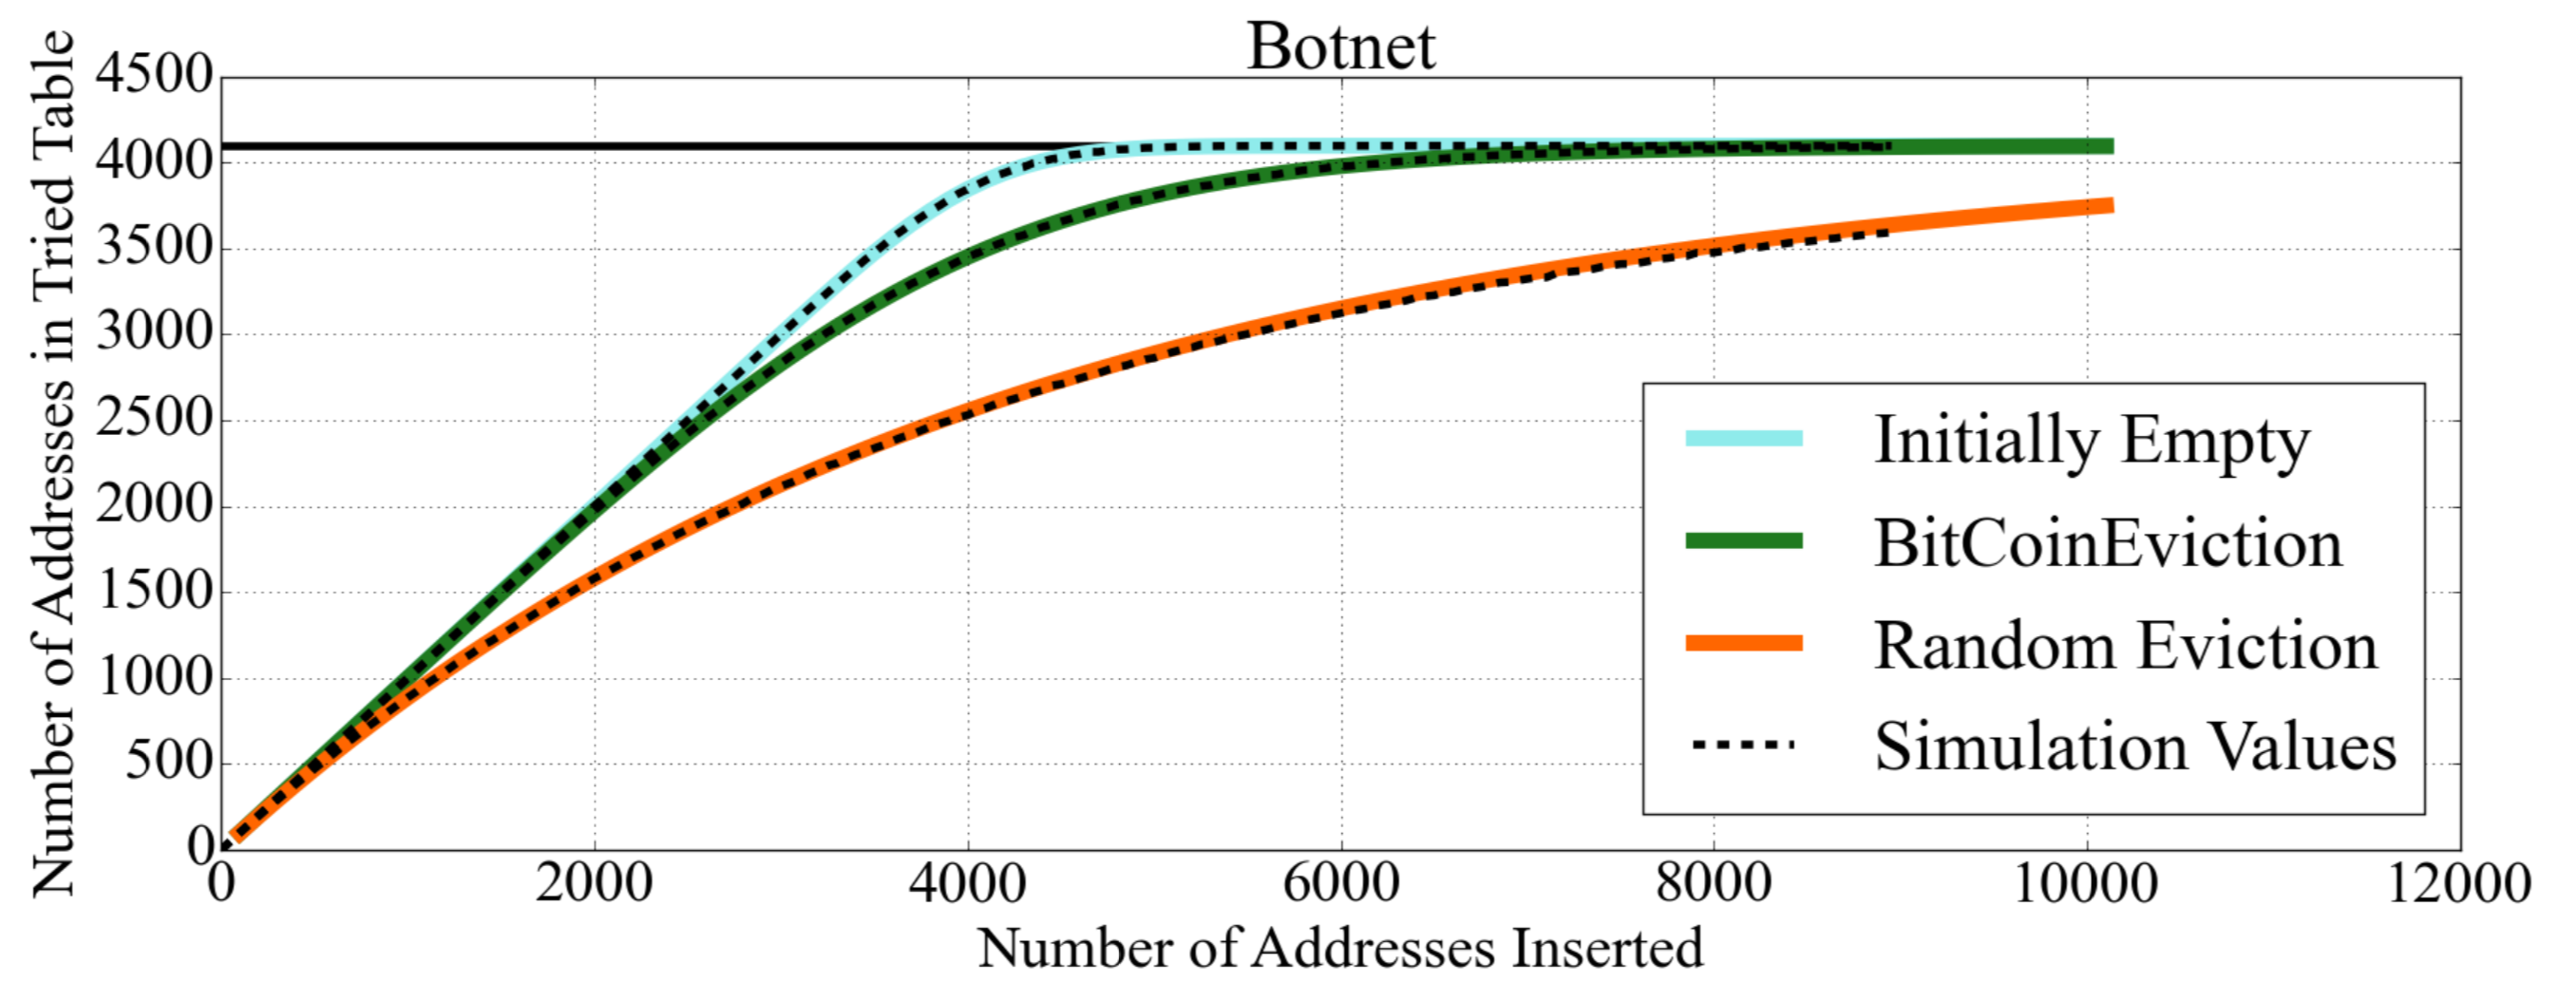
\includegraphics[width=0.85\columnwidth]{images/eclipse-botnet.png}
\caption{Effectivity of a botnet-based eclipse attack \cite{Heilman2015EclipseAO}}
\label{fig:eclipse-botnet}
\end{figure}

\subsection{Countermeasures}

Countermeasures commonly employed by mining pools include disabling incoming connections and using whitelists for outgoing connections. However, these solutions cannot scale to the whole network; in particular, disabling incoming connections would prevent new nodes from joining the network.

The authors suggest several other ways to increase resilience against eclipse attacks.

\begin{itemize}
    \item \textbf{Better address selection and eviction}: On the client-level, changes in address eviction policy and address selection might reduce the probability of the attacker filling the \emph{tried} and \emph{new} tables.
    \item \textbf{Feeler connections}: Special connections could be used to make sure addresses in the \emph{new} table are indeed valid addresses.
    \item \textbf{Anchor connections}: A portion of a node's outgoing connections could be persisted between restarts, making it harder for the attacker to occupy these.
    \item \textbf{Ban large unsolicited ADDR messages}: Nodes might choose to ignore multiple, large ADDR messages sent by peers.
    \item \textbf{Anomaly detection}: By analyzing traffic information and characteristics of the new and \emph{tried} table, it might be possible to detect and address an ongoing eclipse attempt.
\end{itemize}

For a more thorough description of countermeasures, we encourage the reader to refer to the original paper \cite{Heilman2015EclipseAO}.

\section{Partitioning attack}
\label{sec:partitioning}

\subsection{Overview}

The possibility and practicality of partitioning attacks on Bitcoin's peer-to-peer network were demonstrated by Maria Apostolaki, Aviv Zohar, and Laurent Vanbever in 2017 \cite{RoutingAttacks}. In this attack, an AS-level adversary isolates a set of nodes from the rest of the network by interfering with BGP routing. The attack can be used to isolate a small number of nodes or to split the network into two partitions of roughly the same size.

\subsection{Prerequisites}

Partitioning attacks can be executed by AS-level adversaries including ISPs, large corporations, and governments. The attack relies on BGP hijacking, so the attacker needs to be able to participate in BGP routing and announce IP prefixes. As the attack generally does not involve stateful packet inspection, hardware requirements are relatively low.

\subsection{Attack process}

Let us say that the AS-level adversary has identified a set of nodes $P$ it wishes to isolate from the rest of the network. The nodes are identified by their public IP addresses.

The attack involves the following steps (illustrated by figure \ref{fig:partition-attack}):

\begin{enumerate}
    \item \textbf{Divert traffic destined to $P$}: First, the attacker performs a BGP hijack by announcing a set of IP prefixes that covers all nodes in $P$. In order for the attack to be successful, these prefixes need to be more specific than those announced by honest ASes.
    
    For instance, if an honest AS announces the range 100.0.0.0/16, a malicious AS could perform a BGP hijack by announcing two ranges 100.0.0.0/17 and 100.0.0.128/17.
    
The result of this is that all traffic susceptible BGP hijacking to and from nodes in $P$ will be routed through the attacker. 

\begin{figure} [h!]
\centering
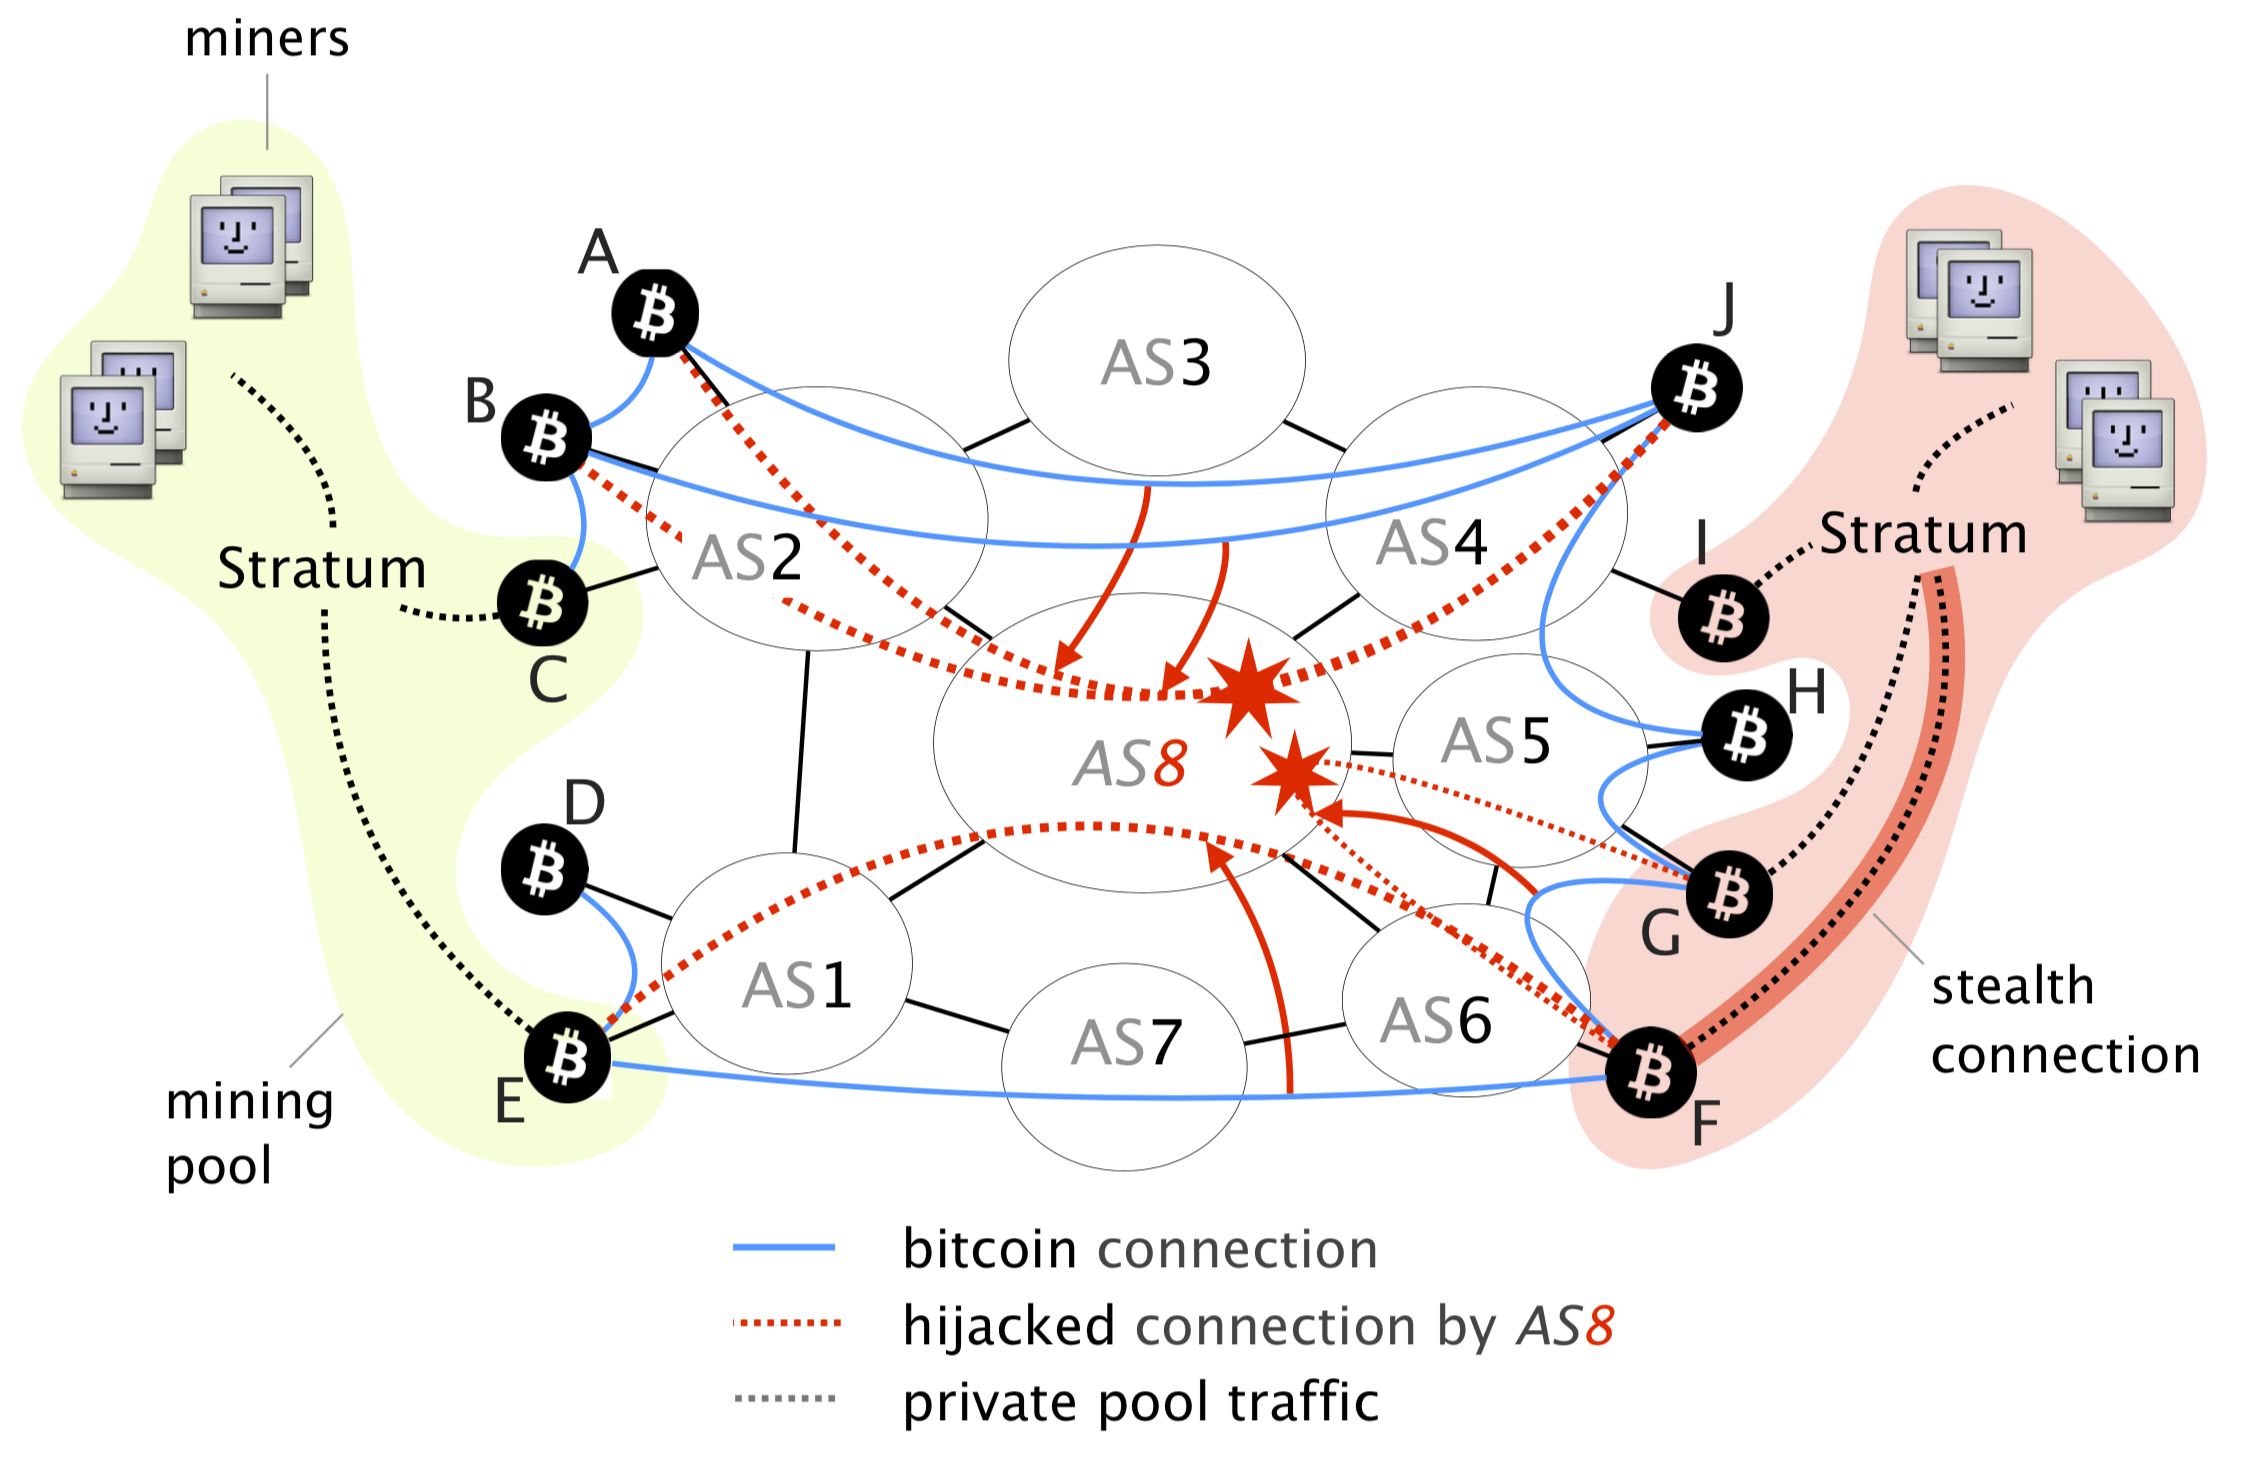
\includegraphics[width=0.8\columnwidth]{images/routing-attack.png}
\caption{An AS-level adversary (AS8) wants to isolate the set of nodes $\{A,B,C,D,E,F\}$ \cite{RoutingAttacks}}
\label{fig:partition-attack}
\end{figure}

    \item \textbf{Identify relevant traffic}: Having rerouted all traffic to and from nodes in $P$ through itself, the attacker then needs to identify Bitcoin traffic. This can easily be done by matching on well-known ports (TCP:8333 for Bitcoin), specific IP addresses, and fields of the unencrypted Bitcoin header.
    
    \item \textbf{Drop packets crossing partition boundary}: At this point, the attacker can partition the network by dropping all Bitcoin packets crossing the boundary.
    
    $$(\textrm{IP}_{from} \in P \land \textrm{IP}_{to} \not\in P) \lor (\textrm{IP}_{from} \not\in P \land \textrm{IP}_{to} \in P)$$

    \item \textbf{Isolate leaking nodes}: The main challenge is to isolate leaking nodes. These are nodes within $P$ that communicate with nodes outside $P$ on routes or channels that cannot be hijacked using BGP. These include
    
    \begin{itemize}
        \item intra-AS traffic, i.e. two nodes within the same AS (figure \ref{fig:stealth}),
        \item intra-pool communication (potentially using non-Bitcoin protocol), and
        \item pool-to-pool communication, i.e. secret peering agreements.
    \end{itemize}
    
\begin{figure}[h!]
\centering
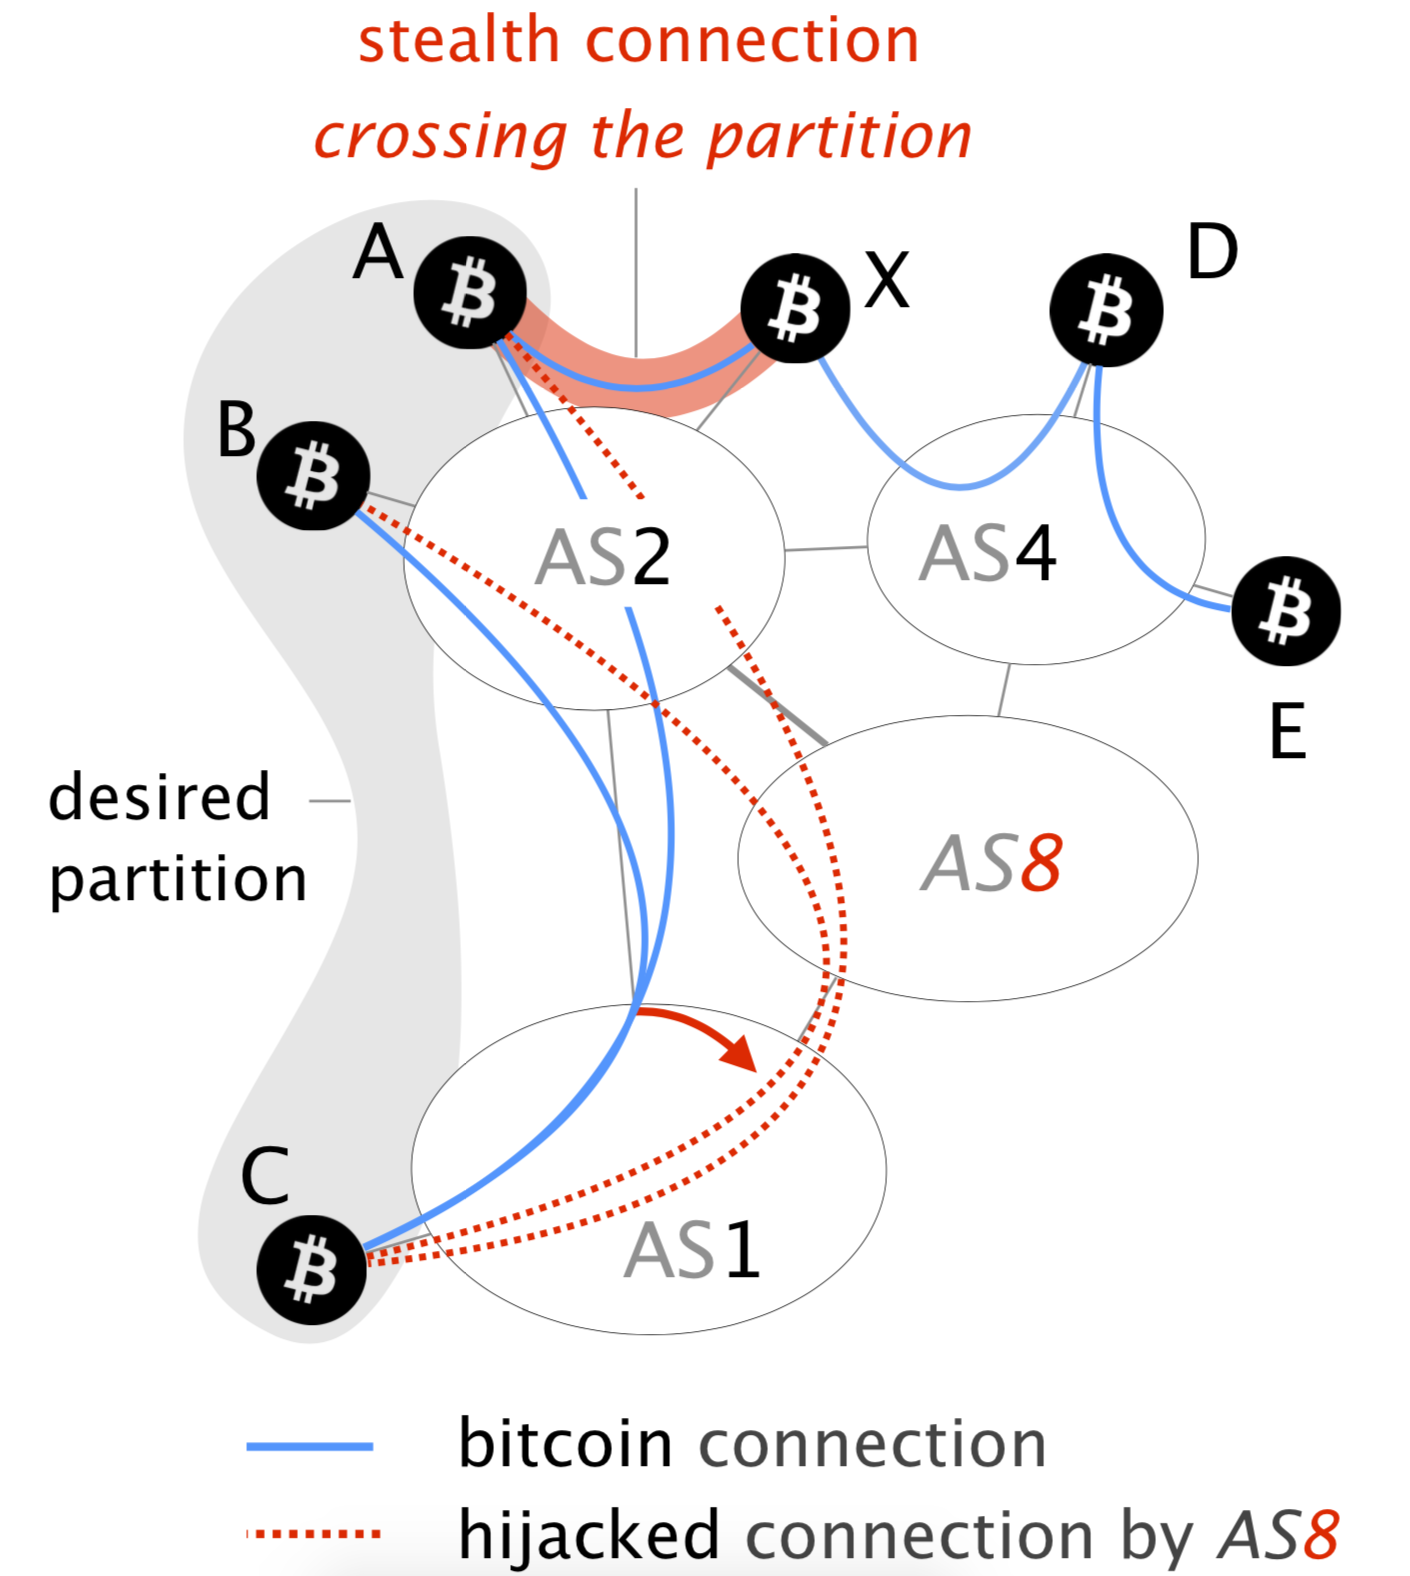
\includegraphics[width=0.45\columnwidth]{images/stealth-connection.png}
\caption{Stealth connection between nodes within the same AS \cite{RoutingAttacks}}
\label{fig:stealth}
\end{figure}
    
    To reduce the chance of such leaks, the attacker can make sure to include either all or none of the nodes from specific ASes and pools. However, such precautions can still leave some stealth connections undetected, essentially defeating the attack.
    
To isolate all leaks, the attacker must monitor INV messages sent from nodes within $P$ and outside $P$.  When a node in $P$ advertises blocks mined outside $P$, it has a stealth connection and must be excluded from $P$. With this process, the attacker can arrive at the maximum feasible subset of $P$ being isolated from the rest of the network.
    
\end{enumerate}

\subsection{Impact and relevance}

A successful partitioning attack can have a serious impact on the nodes involved.

With a targeted attack involving a small group of nodes, the attacker can perform Denial-of-Service, preventing the nodes in $P$ from getting network updates. This is very similar to eclipse attacks, but the attacker in this case uses the network infrastructure itself instead of individual nodes. This attack can be used for other attacks like double spending and selfish mining.

A network-wide partitioning attack could essentially cut the network into two isolated networks, with roughly 50\% hash power each, effectively causing a fork. With reduced hash power, these partitions will be more susceptible to a range of attacks including 51\% attack. In practice, one of the partition will have at least slightly more hash power and will create a longer chain during the time of the attack. As the partitions will rejoin after the attack has finished, all blocks in the shorter chain will be discarded, opening the door to N-confirmation double spend attacks and making the affected miners lose revenue.

The practicality of a targeted attack has been demonstrated by the authors of \cite{RoutingAttacks} by partitioning their own nodes using a virtual AS. Through thorough analysis, the authors made the following observations:

\begin{itemize}
    \item Around 10 ASes host almost 30\% of all Bitcoin nodes, making the network rather centralized on the network infrastructure level.
    \item Around 10 ASes naturally intercept more than 80\% of all Bitcoin traffic.
    \item The authors have been able to divert all traffic to and from their nodes within 90 seconds.
    \item 47\% of mining power can be isolated by hijacking 39 BPG prefixes.
    \item Intentional and accidental hijacks happen all the time, often affecting Bitcoin traffic.
    \item The two partitions can quickly reconnect after the attack but it takes a long time for them to be densely connected again.
\end{itemize}

These characteristics of the Bitcoin network and the Internet infrastructure in general make partitioning attacks feasible. Designers of peer-to-peer networks must keep this in mind and increase the difficulty of executing such attacks by design.

\subsection{Countermeasures}
\label{subsec:part-counter}

The following countermeasures can alleviate some of the risks of partitioning attacks.

\begin{itemize}
    \item \textbf{Prefer connections that cannot be hijacked}: By preferring nodes within the same AS and/or in /24 prefixes, nodes can prevent attackers from diverting all their traffic.

    \item \textbf{Diversity of connections}: Nodes can connect to the internet through multiple ASes. By using an encrypted VPN tunnel, one can prevent an attacker from identifying Bitcoin traffic.

    \item \textbf{Multi-homing}: Mining pools should and often already do have multiple gateways hosted in multiple ASes. Pool-to-pool peering agreements might also help to alleviate the risks.

    \item \textbf{Anomaly detection}: By monitoring traffic properties (routing information with traceroute, Round Trip Time, etc.), nodes can identify hijacks and other potential attacks. For instance, nodes should monitor routes and prevent a single AS from appearing in all paths.
\end{itemize}

Furthermore, protocol-level changes could reduce the risk of successful partitioning attacks significantly. In particular, encrypting Bitcoin traffic, and using randomized ports (or incorporating port negotiation) would make it significantly harder to identify Bitcoin traffic.

\begin{figure} [h!]
\centering
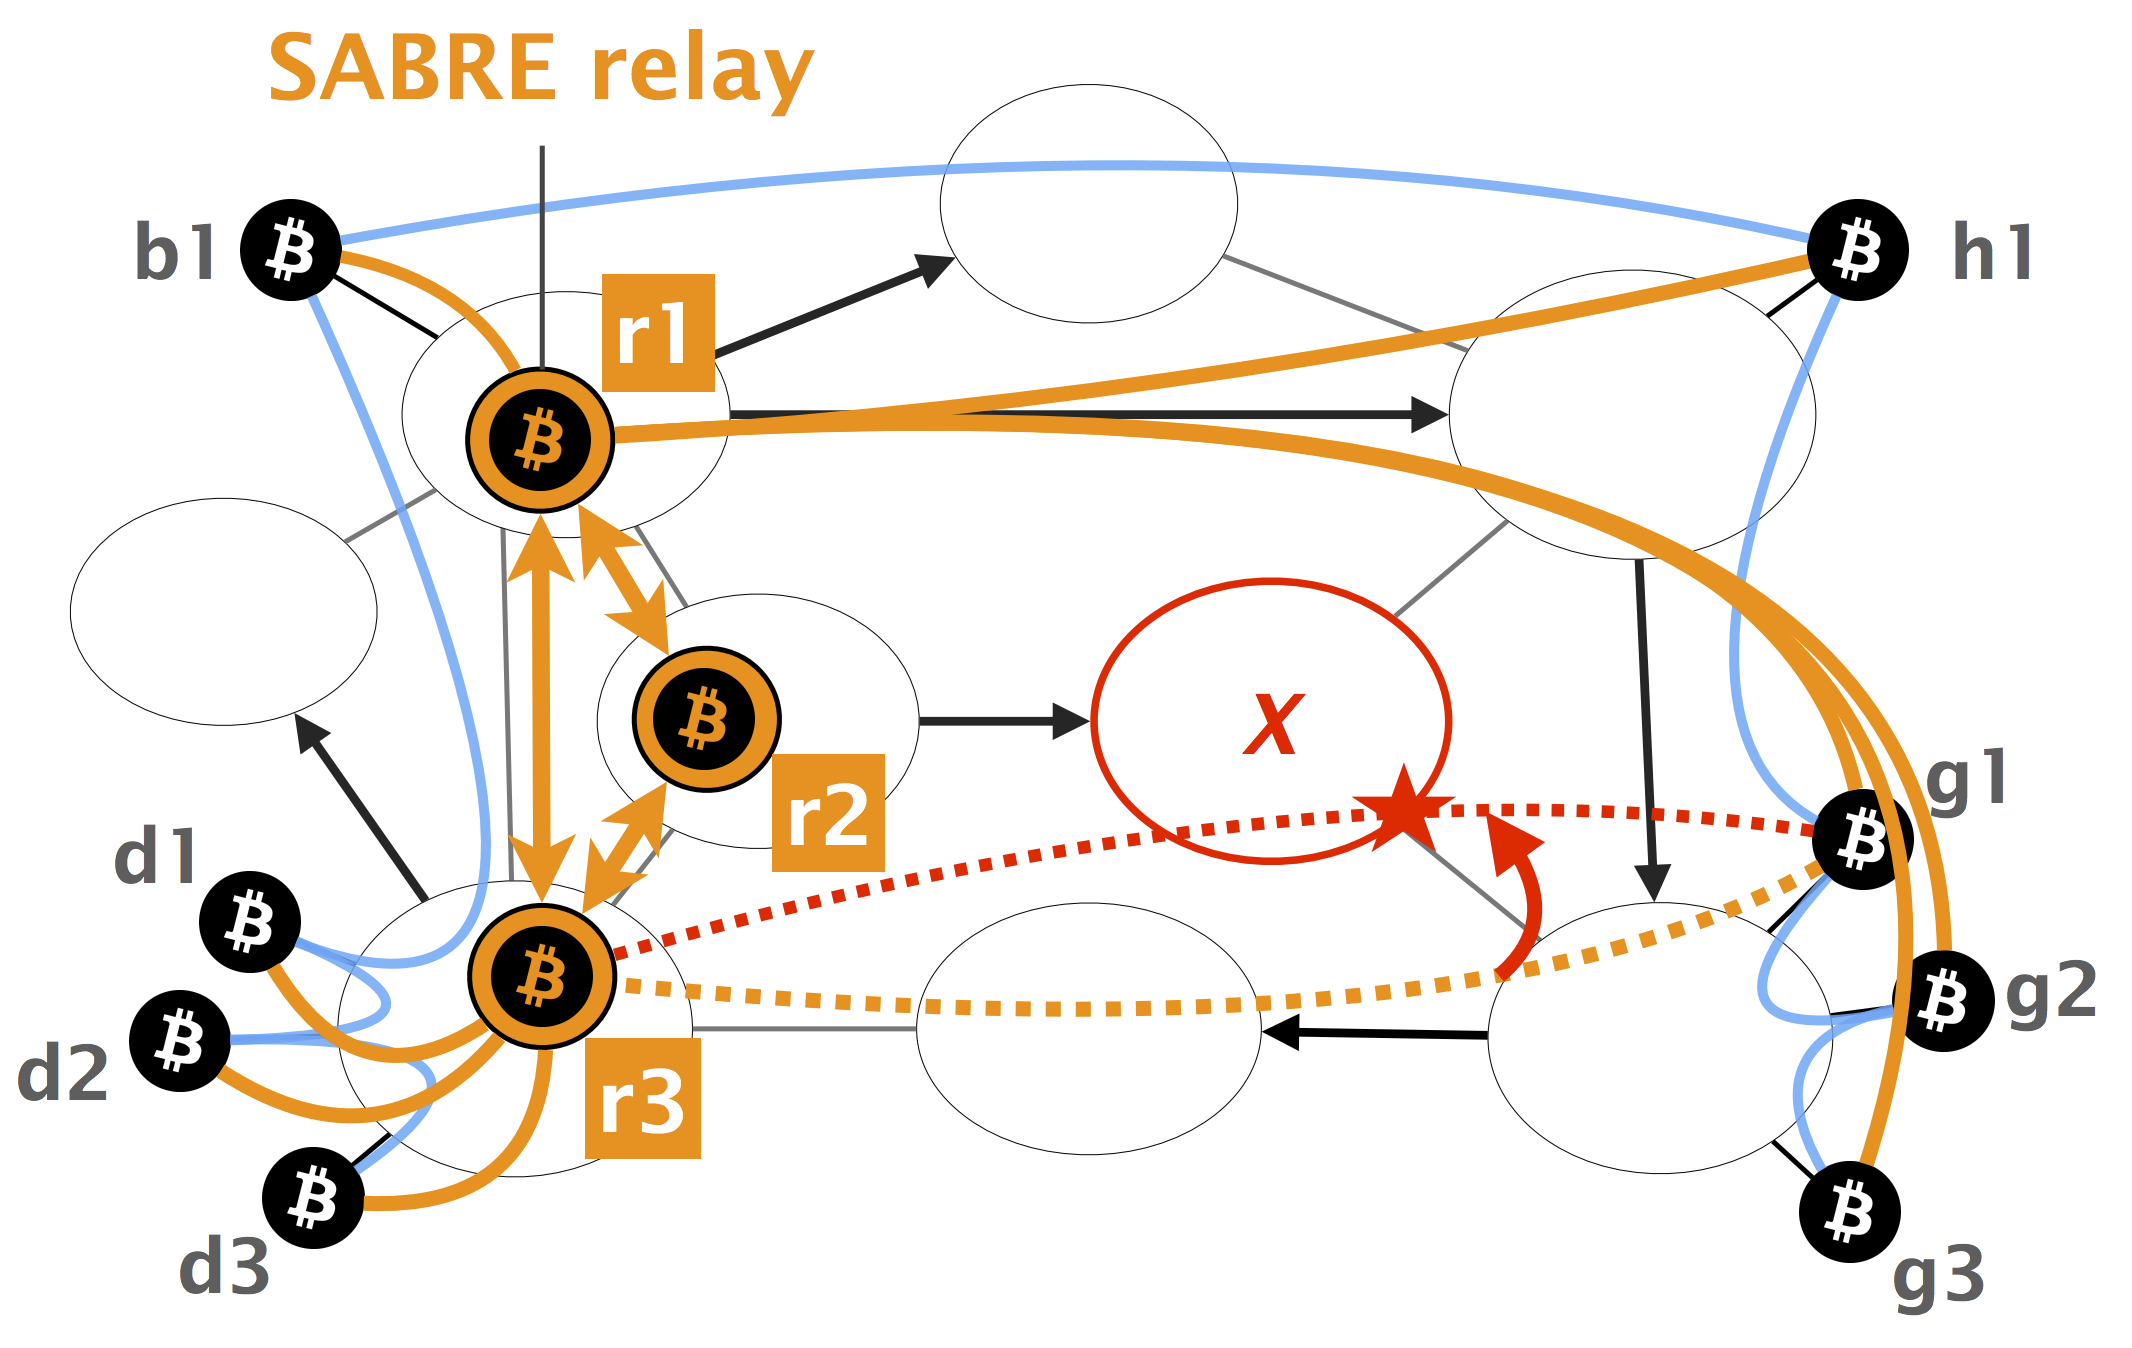
\includegraphics[width=0.7\columnwidth]{images/sabre.png}
\caption{The SABRE overlay network \cite{SABRE}}
\label{fig:sabre}
\end{figure}

Apostolaki et al. designed a system called SABRE, with the aim of making the Bitcoin network more secure (figure \ref{fig:sabre}) \cite{SABRE}. SABRE is a voluntary overlay network designed to be robust and secure. They achieve this using the following steps.

\begin{itemize}
    \item \textbf{Relay-to-relay connections}: Secure connections by hosting nodes in /24 prefixes in ASes with direct peering connections forming a k-connected cluster.

    \item \textbf{Client-to-relay connections}: Reduce the chance of successful BGP hijacks by strategically placing relay nodes so that they will likely be preferred by ASes hosting many Bitcoin nodes.
    
    \item \textbf{Relay-to-client connections}: reduce the chance of successful BGP hijacks by using traffic obfuscation (e.g. change source IP).
    
    \item \textbf{DDoS}: Increase DDoS resistance by using resilient hardware-software co-design.
\end{itemize}

While the Bitcoin community is generally skeptical of such centralized solutions, the authors argue that the voluntary and transparent nature of SABRE will help increase the security of the whole network.

\section{Delay attack}
\label{sec:delay}

\subsection{Overview}

Apostolaki et al. introduced the concept of network infrastructure-level delay attacks in their paper discussing routing attacks \cite{RoutingAttacks}. In this attack, an AS-level adversary hijacks a portion of the in- or outgoing traffic associated with a Bitcoin node and incurs a high message delay by tampering with the packages. The attack can make the node uninformed of the latest blocks for a significant portion of its uptime, potentially leading to revenue loss and opening up the possibility of other attacks.

\begin{figure}
\centering
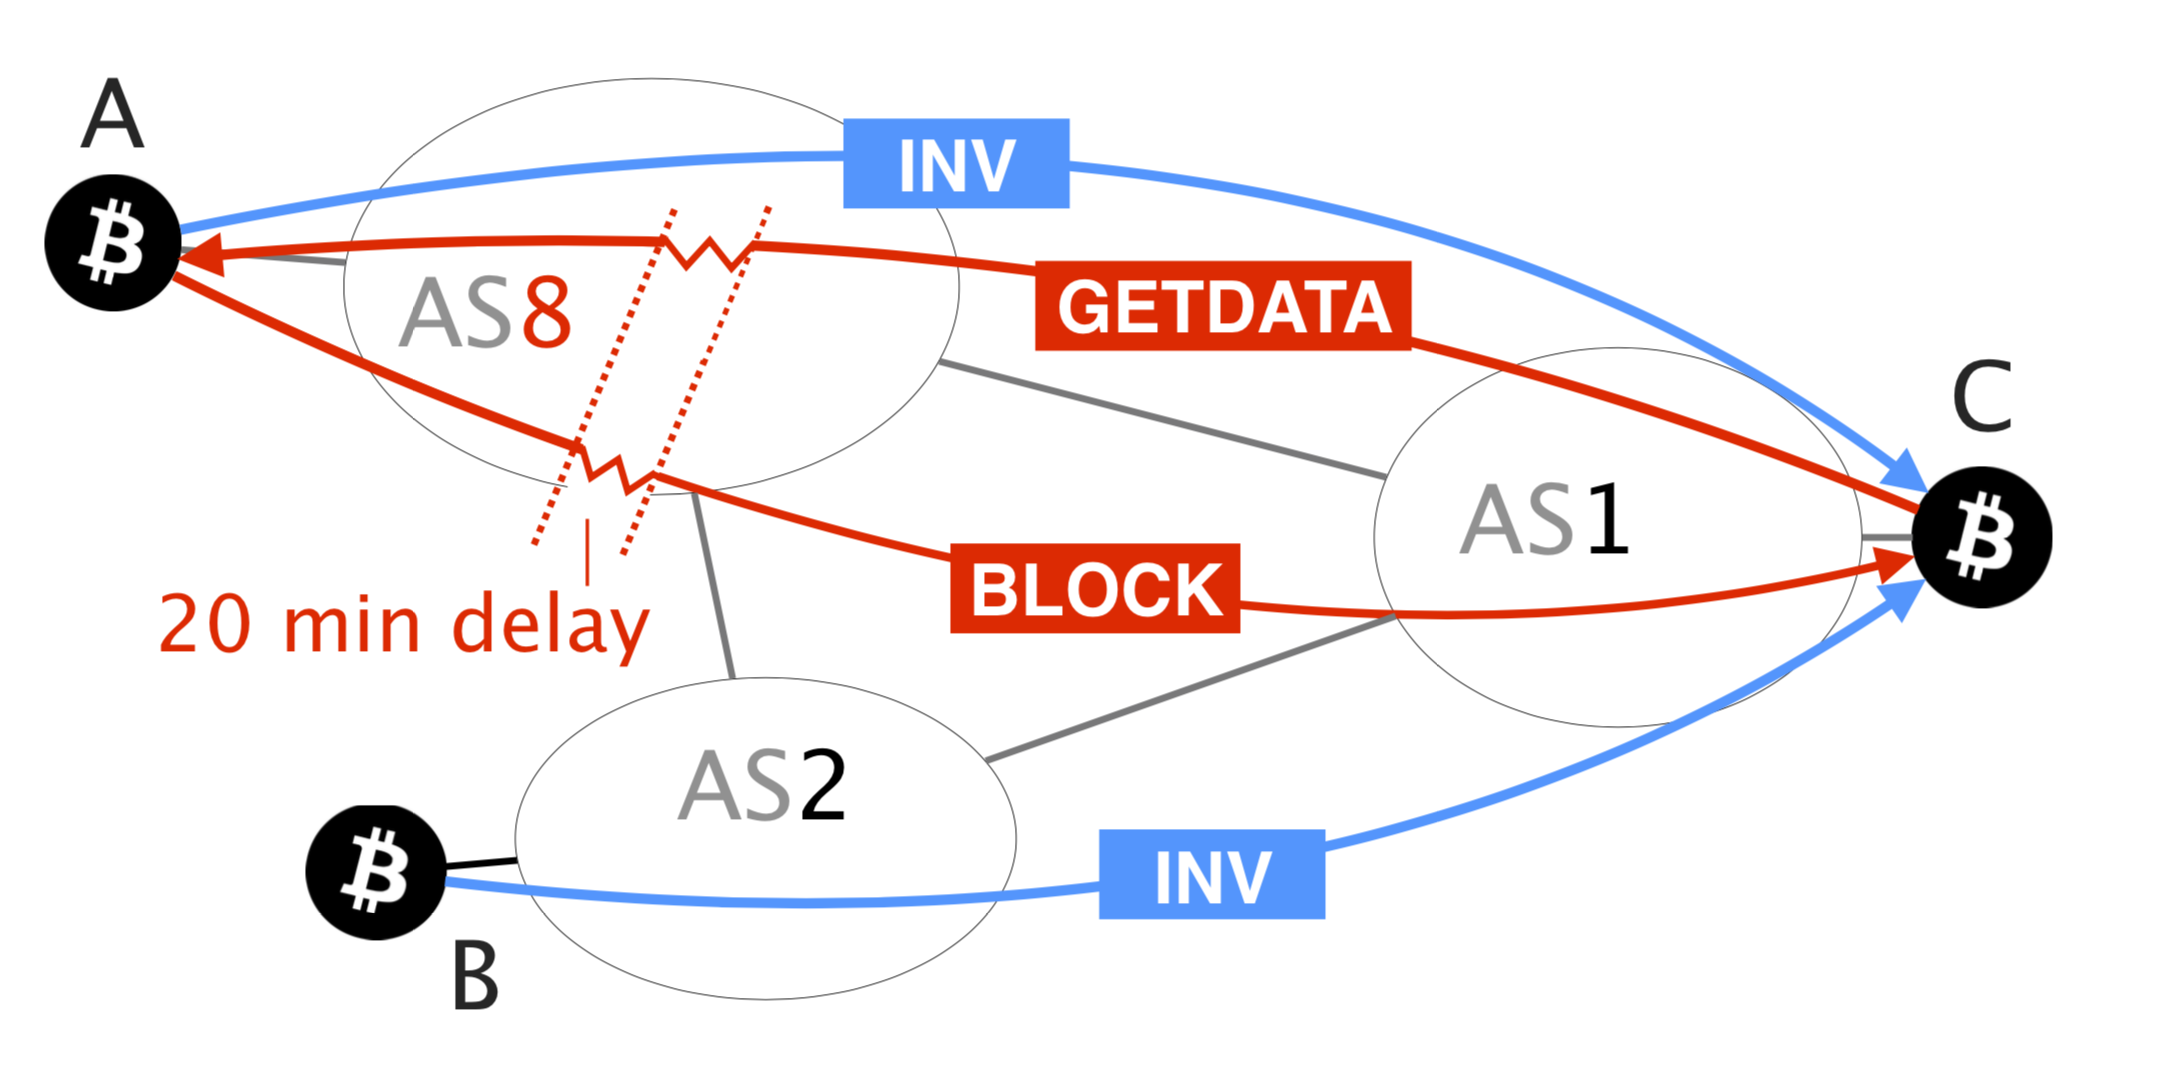
\includegraphics[width=0.6\columnwidth]{images/delay-attack.png}
\caption{Delay attack \cite{RoutingAttacks}}
\label{fig:delay}
\end{figure}

\subsection{Prerequisites}

Delay attacks have similar requirements to those of partitioning attacks. These attacks can be executed by AS-level adversaries including ISPs, large corporations, and governments. The attack relies on BGP hijacking, so the attacker needs to be able to participate in BGP routing and announce IP prefixes. However, the attacker does not need to be able to intercept all traffic in order to succeed. As the attack generally does not involve stateful packet inspection, hardware requirements are relatively low.

\subsection{Attack process}

In a delay attack, the attacker's goal is to prevent the target node from receiving correct information. At the same time, the attacker would preferably want to keep the intercepted connection alive so that she can continue the exploit.

In contrast to partitioning attacks (section \ref{sec:partitioning}), an attacker performing a delay attack does not need to intercept all traffic associated with a node. However, by increasing the portion of traffic intercepted, the attacker can make the node stay uninformed for a bigger portion of its uptime.

BGP hijacks might, in some cases, only affect one direction of a bi-directional TCP connection. Thus, we will follow \cite{RoutingAttacks}'s discussion and describe the attack in two cases: intercepting outgoing connections and intercepting incoming connections.

\begin{figure}
\centering
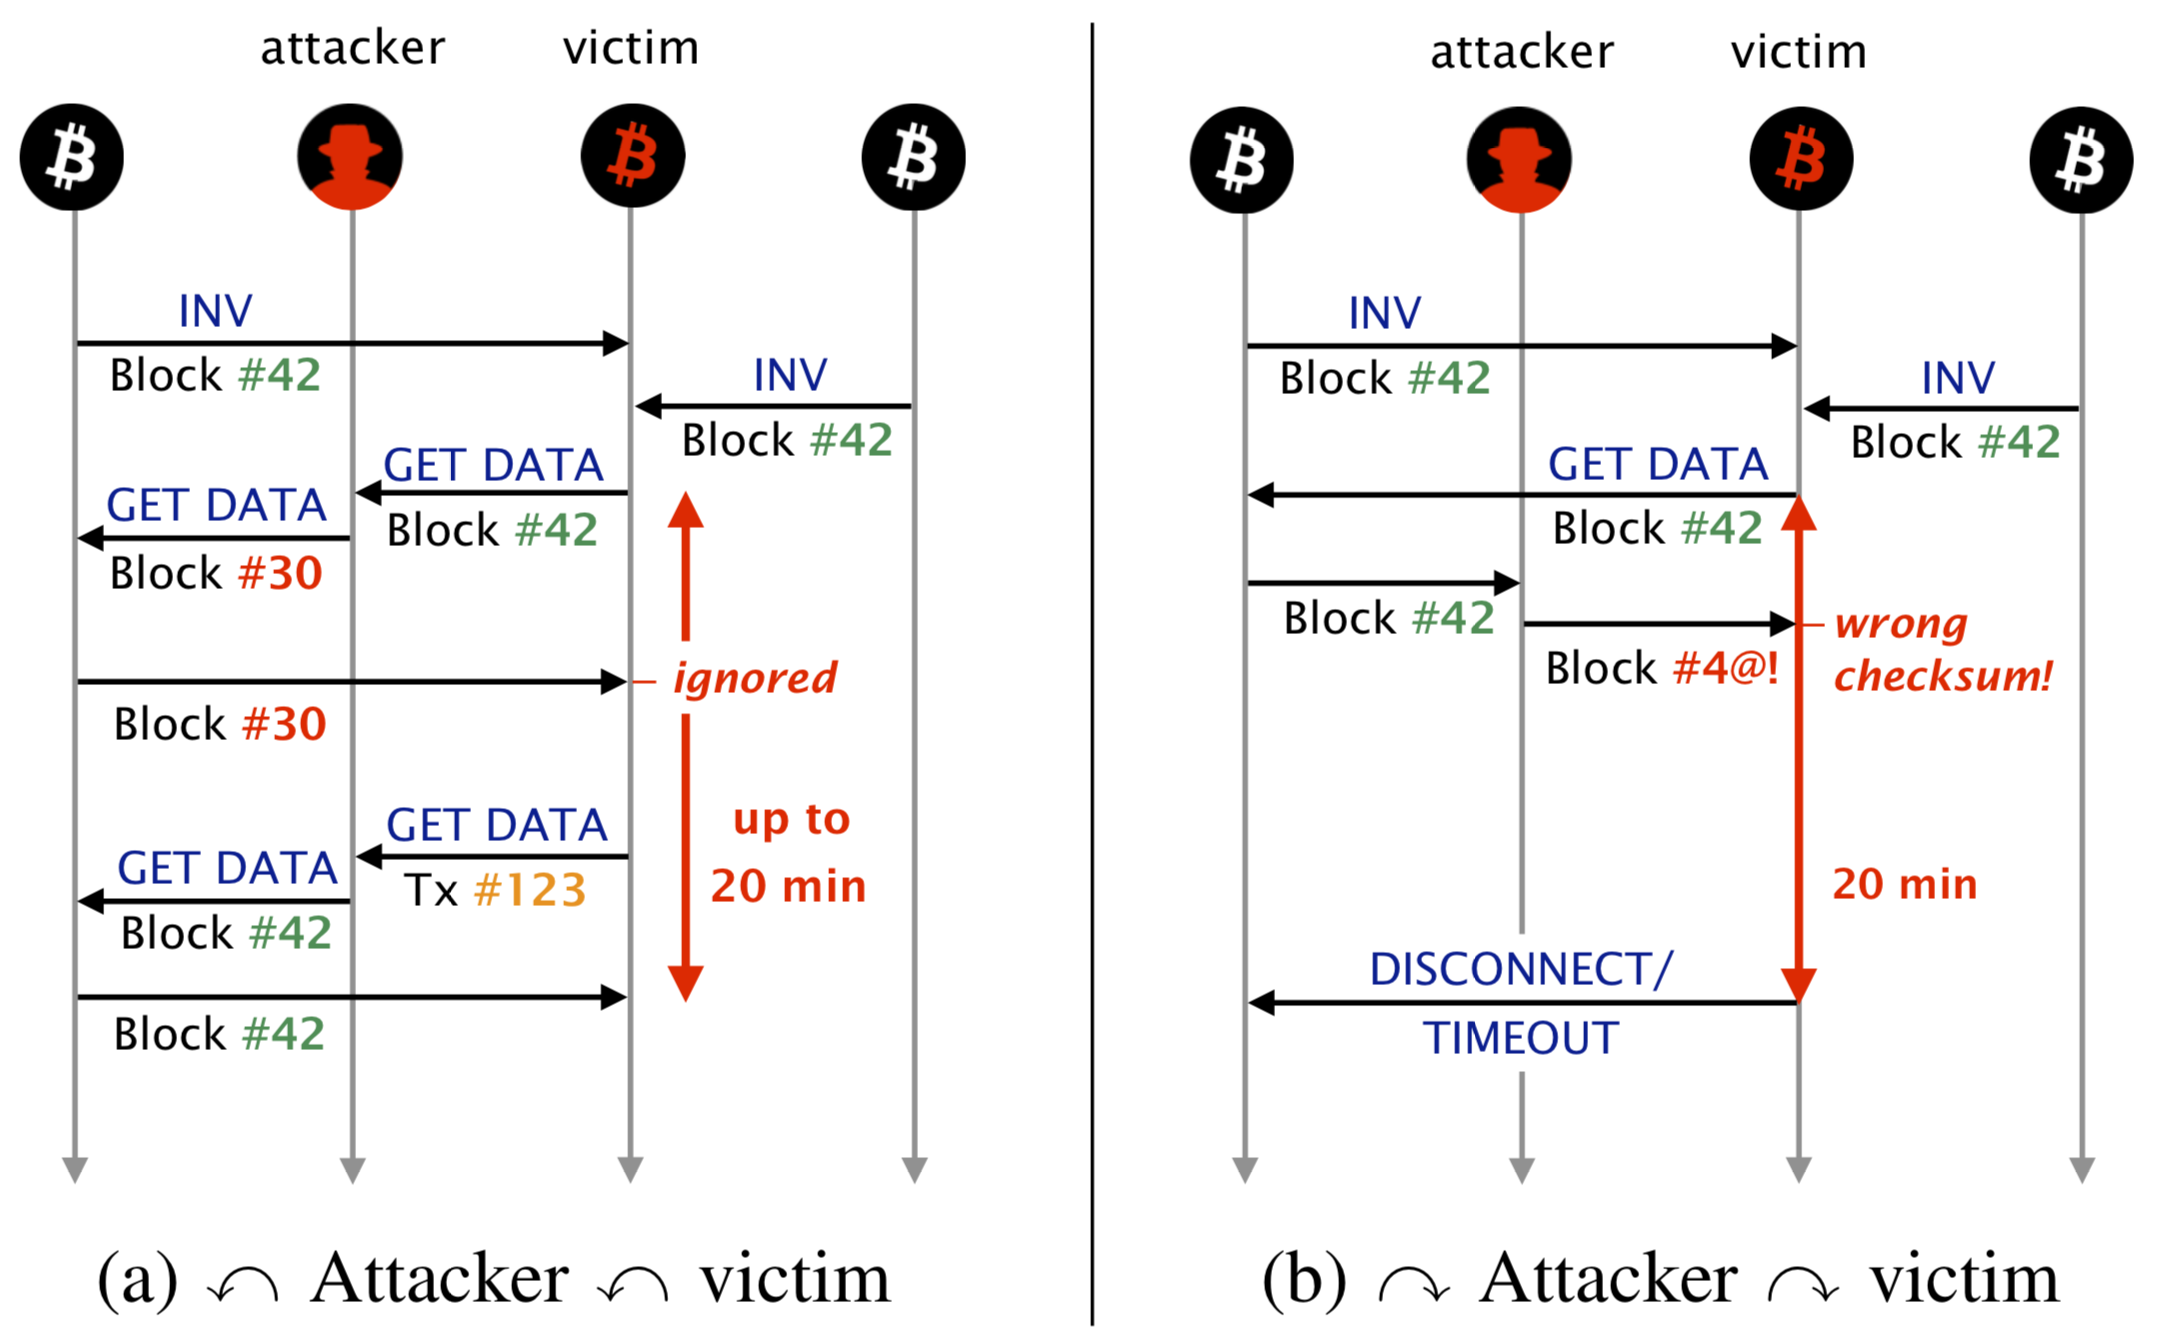
\includegraphics[width=0.8\columnwidth]{images/delay-attack-detailed.png}
\caption{Example of a delay attack for (a) outgoing, and (b) incoming connections \cite{RoutingAttacks}}
\label{fig:delay-detailed}
\end{figure}

\subsubsection{Intercept outgoing connection}

First, let us discuss the case when the attacker can intercept a connection from a node to its neighbor, but not the other way around (figure \ref{fig:delay-detailed} (a)).

\begin{enumerate}
	\item \textbf{Perform BGP hijack}: The attacker first performs a BGP hijack with an IP prefix covering the target node. If the attacker announces a prefix that has been announced by an honest AS previously, it will on average intercept 50\% of the traffic to and from the node.
	
	\item \textbf{Tamper with GETDATA}: Nodes periodically receive INV messages from their neighbors. If an INV message contains a block hash that the node is not aware of (i.e. a new block), the node will request this block from the first neighbor that advertised the block using a GETDATA message.
	
Let us assume that the attacker intercepts a GETDATA message requesting block $A$. Given that Bitcoin traffic has no integrity checks apart from message length and checksum, the attacker can secretly change the block hash requested to another (older) block called $B$.

The neighbor then will proceed to send block $B$ to the target node, who in turn will ignore the message and keep waiting for block $A$ for up to 20 minutes.

	\item \textbf{Wait for some time}: At this point, the attacker makes the node wait for as long as possible, without reaching the end of the 20-minute timeout.

	\item \textbf{Intercept another GETDATA message from the node}: Before the end of the timeout, the attacker intercepts another GETDATA message requesting transaction $C$ from the same neighbor. (Note that requesting transaction data is much more common than requesting block data.)

The attacker can change the message content from transaction $C$ to block $A$. The neighbor will proceed to send block $A$ to the target node. As the node received the block within the 20-minute timeout, the connection is kept alive.

The attacker does not drop the message and instead makes sure that the node receives the correct response with a delay of up to 20 minutes. This way, the connection intercepted by the attacker remains open and she can continue her exploit.

\end{enumerate}

\subsubsection{Intercept incoming connection}

Second, let us discuss the case when the attacker can intercept a connection from the neighbor to the node, but not the other way around (figure \ref{fig:delay-detailed} (b)).

\begin{enumerate}
	\item \textbf{Perform BGP hijack}: The attacker first performs a BGP hijack with an IP prefix covering the target node.
	
	\item \textbf{Tamper with BLOCK message}: This time, the attacker cannot intercept the GETDATA message requesting block $A$. However, it can intercept the reply from the neighbor, a BLOCK message containing block $A$'s data.
	
The attacker can tamper with this message to make it invalid and rejected by the target node (e.g. due to checksum mismatch). After this, the node will keep waiting for 20 minutes for a valid BLOCK message.

	\item \textbf{Wait for some time}: At this point, the attacker waits until the end of the 20-minute timeout, at which point the connection is dropped and the node attempt connecting to a new peer.
\end{enumerate}

This attack is less effective than the previous case, as the attacker cannot keep the connection open. However, this still results in a 20-minute delay in block propagation.

\subsection{Impact and relevance}

A successful delay attack can have serious impact on the nodes involved.

With a targeted attack involving a single node, the attacker can perform Denial-of-Service, delaying the node's access to network updates. This can cause the node to mine \emph{on the wrong block}, causing revenue loss and basically excluding the node from the mining process. The attack can also be used for performing other attacks like double spending.

Network-wide delay attacks would have a severe impact on the usability of the system, leading to loss of revenue and trust, with potentially devastating consequences. However, the authors' analysis suggests that network-wide delay attacks are not practical and therefore do not pose a realistic threat to Bitcoin's network.

The authors also demonstrate the following insights:

\begin{enumerate}
    \item Intercepting 50\% of a node's connections can keep it uninformed for 63.32\% of the time.
    \item With an average multi-homing degree of 5, even if all ASes in the US would collude to attack the network, the orphan rate could still only be increased by 5\%.
\end{enumerate}

\subsection{Countermeasures}

Countermeasures discussed in section \ref{subsec:part-counter} apply here as well. In particular, the integration of statistical analysis of network traffic and anomaly detection could help detecting and alleviating delay attacks. Intuitively, a sudden increase in block delay might be indicative of an attack going on.

Protocol-level changes might drastically reduce the risk of a delay attack. Incorporating integrity checks into the Bitcoin network protocol would make it practically impossible to tamper with Bitcoin traffic. By requesting new blocks on multiple connections simultaneously, nodes can also reduce risk.


\section{Conclusions}
\label{sec:conclusion}

We discussed three types of attacks on Bitcoin's peer-to-peer network: Eclipse attacks, partitioning attacks, and delay attacks. While our main focus was on blockchain systems, studying these attacks offers insights for other peer-to-peer systems as well. We believe that by analyzing these attacks, designers of any peer-to-peer systems can gain a deeper understanding of potential attack vectors on their systems. By being aware of these attack vectors, systems can be architected to be secure by design.

% In setting up this template for *Science* papers, we've used both
% the \section* command and the \paragraph* command for topical
% divisions.  Which you use will of course depend on the type of paper
% you're writing.  Review Articles tend to have displayed headings, for
% which \section* is more appropriate; Research Articles, when they have
% formal topical divisions at all, tend to signal them with bold text
% that runs into the paragraph, for which \paragraph* is the right
% choice.  Either way, use the asterisk (*) modifier, as shown, to
% suppress numbering.


% Your references go at the end of the main text, and before the
% figures.  For this document we've used BibTeX, the .bib file
% scibib.bib, and the .bst file Science.bst.  The package scicite.sty
% was included to format the reference numbers according to *Science*
% style.

\bibliographystyle{unsrt}

\begin{thebibliography}{99}

\bibitem{BitTorrent} Johnsen, J.A. (2005). Peer-to-peer networking with BitTorrent.

\bibitem{IPFS} Benet, J. (2014). IPFS - Content Addressed, Versioned, P2P File System. CoRR, abs/1407.3561.

\bibitem{SignalSecurity} Cohn-Gordon, K., Cremers, C.J., Dowling, B., Garratt, L., \& Stebila, D. (2016). A Formal Security Analysis of the Signal Messaging Protocol. 2017 IEEE European Symposium on Security and Privacy (EuroS\&P), 451-466.

\bibitem{TOR} Dingledine, R., Mathewson, N., Murdoch, S.T., \& Murdoch, S. (2014). Tor: The Second-Generation Onion Router (2014 DRAFT v1).

\bibitem{Nakamoto2008} Nakamoto, Satoshi. (2008). Bitcoin: A Peer-to-Peer Electronic Cash System.

\bibitem{P2PSecurityTaxonomy} Ferdous, Md. S., Chowdhury, F. \& Moniruzzaman, Md. (2007). A Taxonomy of Attack Methods on Peer-to-Peer Network. 1st Indian Conference on Computational Intelligence and Information Security, 2007 (ICCIIS, 07), 132-138.

\bibitem{P2PAttacks} Helsinki, L.W. (2006). Attacks Against Peer-to-peer Networks and Countermeasures.

\bibitem{P2PAttacks2} Prêtre, B., Wattenhofer, R., \& Schmid, S. (2006). Attacks on Peer-to-Peer Networks.

\bibitem{Byzantine} Pease, M.C., Shostak, R.E., \& Lamport, L. (1980). Reaching Agreement in the Presence of Faults. J. ACM, 27, 228-234.

\bibitem{FLP} Fischer, M.J., Lynch, N.A., \& Paterson, M. (1983). Impossibility of Distributed Consensus with One Faulty Process. PODS.

\bibitem{PBFT} Castro, M.O. (1999). Practical Byzantine Fault Tolerance. OSDI.

\bibitem{Garam} Garamvölgyi, P. (2017). Blockchain-based control of device access in cyber-physical systems.

\bibitem{GHOST} Sompolinsky, Y., \& Zohar, A. (2015). Secure High-Rate Transaction Processing in Bitcoin. Financial Cryptography.

\bibitem{Incentives} Yao, A.C. (2018). An Incentive Analysis of some Bitcoin Fee Designs. CoRR, abs/1811.02351.

\bibitem{PoS} King, S., \& Nadal, S. (2012). PPCoin : Peer-to-Peer Crypto-Currency with Proof-of-Stake.

\bibitem{PoS2} Buterin, V., \& Griffith, V. (2017). Casper the Friendly Finality Gadget. CoRR, abs/1710.09437.

\bibitem{Inclusive} Lewenberg, Y., Sompolinsky, Y., \& Zohar, A. (2015). Inclusive Block Chain Protocols. Financial Cryptography.

\bibitem{SPECTRE} Sompolinsky, Y., Lewenberg, Y., \& Zohar, A. (2016). SPECTRE: A Fast and Scalable Cryptocurrency Protocol. IACR Cryptology ePrint Archive, 2016, 1159.

\bibitem{GHOSTDAG} Sompolinsky, Y. (2018). PHANTOM , GHOSTDAG : Two Scalable BlockDAG protocols.

\bibitem{Conflux} Li, C., Li, P., Xu, W., Long, F., \& Yao, A.C. (2018). Scaling Nakamoto Consensus to Thousands of Transactions per Second. CoRR, abs/1805.03870.

\bibitem{Tangle} Popov, S. (2015). The tangle.

\bibitem{Avalanche} Team Rocket. (2018). Snowflake to Avalanche: A Novel Metastable Consensus Protocol Family for
Cryptocurrencies.

\bibitem{SelfishMining} Eyal, I., \& Sirer, E.G. (2014). Majority is not enough: bitcoin mining is vulnerable. Commun. ACM, 61, 95-102.

\bibitem{BitcoinWeaknesses} Bitcoin Wiki, Weaknesses, https://en.bitcoin.it/wiki/Weaknesses

\bibitem{Heilman2015EclipseAO} Heilman, E., Kendler, A., Zohar, A., \& Goldberg, S. (2015). Eclipse Attacks on Bitcoin's Peer-to-Peer Network. IACR Cryptology ePrint Archive, 2015, 263.

\bibitem{RoutingAttacks} Apostolaki, M., Zohar, A., \& Vanbever, L. (2017). Hijacking Bitcoin: Routing Attacks on Cryptocurrencies. 2017 IEEE Symposium on Security and Privacy (SP), 375-392.

\bibitem{BitcoinNetwork} Bitcoin Wiki, Network, https://en.bitcoin.it/wiki/Network

\bibitem{EthereumEclipse} Marcus, Y., Heilman, E., \& Goldberg, S. (2018). Low-Resource Eclipse Attacks on Ethereum's Peer-to-Peer Network. IACR Cryptology ePrint Archive, 2018, 236.

\bibitem{SABRE} Apostolaki, M., Marti, G., Müller, J., \& Vanbever, L. (2018). SABRE: Protecting Bitcoin against Routing Attacks. CoRR, abs/1808.06254.

\end{thebibliography}

\end{document}